\documentclass[12pt]{jreport}
\usepackage{comment}
\usepackage{./sty/eclepsf}
\usepackage{tascmac}
\usepackage{tabularx}
\usepackage{listliketab}
\usepackage[longnamesfirst]{natbib}
\usepackage[dvipdfmx]{graphics}
\usepackage[dvipdfmx]{graphicx}
\usepackage[dvipdfmx]{color}
\usepackage{subfigure}
\usepackage{alltt}
\usepackage{here}
\usepackage{afterpage}
\usepackage{./sty/ncodeline}
%\usepackage[dvipdfmx, colorlinks, breaklinks,%
\usepackage[dvipdfmx, breaklinks,%
bookmarks=true, bookmarksnumbered=true,%
bookmarkstype=toc, bookmarksopen=true,bookmarksopenlevel=3,%
pdftitle={RG},%
]{hyperref}
\usepackage{bookmark}

\AtBeginDvi{\special{pdf:tounicode EUC-UCS2}}

\usepackage{fancyhdr}

\usepackage{./sty/doxygenorig}

\usepackage{indentfirst}
\usepackage{url}
\usepackage{listings,./sty/jlisting}

\def\lstlistingname{プログラム}

\lstset{%
 language={C++},
 %backgroundcolor={\color[gray]{.85}},%
 basicstyle={\small\ttfamily},%
 identifierstyle={\small},%
 commentstyle={\small\itshape},%
 keywordstyle={\small\bfseries},%
 ndkeywordstyle={\small\ttfamily},%
 stringstyle={\small\ttfamily},
 frame={tb},
 framesep=1zw,
 breaklines=true,
 numbers=left,%
 xrightmargin=0zw,%
 xleftmargin=1.5zw,%
 numberstyle={\scriptsize},%
 stepnumber=1,
 numbersep=1zw,%
 lineskip=-0.5ex%
}

\usepackage{amssymb}
%\usepackage{supertabular,multirow}

\usepackage{array}
\newcolumntype{M}[1]{>{\centering\arraybackslash}m{#1}}

% A4  size: 297mm*210mm %1pt = 0.35mm
\setlength{\topmargin}{-3.4mm} % 10pt 25.4mm - 3.4mm = 22mm
\setlength{\oddsidemargin}{-0.4mm} % 25.4mm - 0.4mm = 25mm
\setlength{\evensidemargin}{-0.4mm} % 25.4mm - 0.4mm = 25mm
\setlength{\textheight}{231mm} % 660pt % original is 225.75mm 645pt
\setlength{\textwidth}{160mm} % 457pt

\renewcommand{\topfraction}{.99}
\renewcommand{\textfraction}{.0}
\renewcommand{\floatpagefraction}{.99}
\renewcommand{\bibname}{参考文献}


% \pagestyle{fancy}
\lhead[]{}

\makeatletter
\def\chaptermark#1{\markboth {\ifnum \c@secnumdepth>\m@ne
\@chapapp\ \thechapter \@chappos\ \fi #1}{}}
\makeatother

% タイトル
\def\title{骨格推定を用いたボディビルのポージング練習ツール}
% 英語タイトル
\def\etitle{Bodybuilding posing practice tool using pose estimation}
% 著者(日本語)
\def\author{田崎和輝}
% 著者(英語)
\def\eauthor{Kazuki Tasaki}
% 学部・研究科
\def\dept{慶應義塾大学 環境情報学部}
% 学部・研究科(英語)
\def\edept{Keio University Faculty of Environment and Information Studies}

\begin{document}

\pagenumbering{roman}
\begin{titlepage}
  \begin{center}
    \begin{large}
      卒業論文   2023年度(令和05年)\\
      \vspace{24pt}
      \title
      \end{large}
  \end{center}
  \vspace{40em}
  \begin{flushright}
    \large \dept\\
    \author
  \end{flushright}
\end{titlepage}

\thispagestyle{empty}


卒業論文要旨 - 2023年度 (令和05年度)
\begin{center}
\begin{large}
\begin{tabular}{|M{0.97\linewidth}|}
    \hline
      \title \\
    \hline
\end{tabular}
\end{large}
\end{center}

~ \\
  ボディビルをはじめとするフィットネス大会に出場する人は増加傾向にある。日本ボディビル・フィットネス連盟(JBBF)の登録選手数は2015年の2213人から2021年の5576人へと2倍位以上に増加している\cite{jbbf}。
  しかしながら、ボディビル大会への出場は敷居が高く、トレーニング、減量だけでなくステージでの見栄えを良くするためにポージング練習も必須となる。
  ポージング練習は初心者一人で行うのは難しく、トレーナーに指導を受けるという方法があるが高額である。
  本研究では、骨格推定ライブラリであるOpenPoseを用いてカメラの入力から理想のポーズとの関節角度を比較し、視覚的にフィードバックを返すシステムを構築した。

~ \\
キーワード:\\
\underline{1. Bodybuilding},
\underline{2. Posing},
\underline{3. Pose estimation},
\begin{flushright}
\dept \\
\author
\end{flushright}

\thispagestyle{plain}
\clearpage

Abstract of Bachelor's Thesis - Academic Year 2023
\begin{center}
\begin{large}
\begin{tabular}{|p{0.97\linewidth}|}
    \hline
      \etitle \\
    \hline
\end{tabular}
\end{large}
\end{center}

~ \\
The number of people competing in bodybuilding and other fitness competitions is on the rise. The number of registered competitors in the Japan Bodybuilding and Fitness Federation (JBBF) has more than doubled from 2,213 in 2015 to 5,576 in 2021.\cite{jbbf}
Success in bodybuilding competitions depends on a variety of important factors, including weight training, posing skills, and weight loss.

Of the various elements, posing is particularly challenging for beginners to learn on their own. One of the main obstacles for beginners in learning posing practice is that it is difficult to practice alone.
In this case, they may consider receiving instruction from others, such as a personal trainer, but in many cases, the cost is prohibitive and not all beginners have access to such instruction.
To solve this problem, we have developed a posing practice tool that uses skeletal estimation technology.

This system uses a skeletal estimation library called MediaPipe Pose to recognize the user's pose from the camera input and compare the joint angles with the ideal pose.
The system provides real-time audio feedback on the difference in joint angles from the ideal pose, and we believed that the system could enable beginners to improve their posing skills and acquire poses on their own.

The results of the experiment showed that although some subjects were able to improve their poses by using the system, it was not statistically superior.
Comparison of practice methods also failed to show a statistically significant difference compared to practice with mirrors, so we plan to increase the number of samples and the amount of practice, and to improve the system for future verification. If the usefulness of this system can be demonstrated, the results of this study are expected to help reduce the burden on beginners in bodybuilding posing practice.

  ~ \\
Keywords : \\
\underline{1. Bodybuilding},
\underline{2. Posing},
\underline{3. Pose estimation},
\begin{flushright}
\edept \\
\eauthor
\end{flushright}

\thispagestyle{plain}
\clearpage

\tableofcontents\thispagestyle{plain} %目次
\clearpage
\listoffigures\thispagestyle{plain} %図目次
\clearpage
\listoftables\thispagestyle{plain} %表目次
\clearpage

\pagenumbering{arabic}
\chapter{序論}
\label{introduction}

\section{はじめに}
\label{introduction:background}
ボディビルをはじめとするフィットネス大会に出場する人は増加傾向にある。日本ボディビル・フィットネス連盟(JBBF)の登録選手数は2015年の2213人から2022年の5701人へと2倍位以上に増加している\cite{jbbf}。
しかしながら、ボディビル大会への出場は敷居が高く、トレーニング、減量だけでなくステージでの見栄えを良くするためにポージング練習も必須となる。
ポージング練習は初心者単独で行うのは難しく、トレーナーに指導を受けるという方法があるが高額である。
本研究では、骨格推定ライブラリであるOpenPoseを用いてカメラの入力から理想のポーズとの関節角度を比較し、音声フィードバックを返すシステムを構築した。
% ボディビルをはじめとするフィットネス大会に出場する人は増加傾向にある。日本ボディビル・フィットネス連盟(JBBF)の登録選手数は2015年の2213人から2022年の5701人へと2倍位以上に増加している\cite{jbbf}。
% しかしながら、ボディビルではトレーニングや、減量、日焼け、ポージングなどやることが多く、初心者にはハードルが高い部分がある。

筆者は2020年から慶應のバーベルクラブというボディビルをはじめとしたフィットネスの大会に出場するサークルに所属し、ボディビル競技を行っている。トレーニングや減量に関しては、YouTubeなどを用いてステージでの見栄えを良くするためにポージング練習も必須である。しかしながら,2020年は新型コロナウィルスの影響で他者とトレーニングを行うことやポージングレッスンに参加することが困難であった。そのため、自宅でのポージング練習を行うことが多くなった。ボディビル大会への出場経験がない中での単独でのポージング練習はステージで評価されるようなポーズへ近づいているという練習の効果を実感することが難しかった。
% 練習方法としては鏡を使った練習や動画、写真に撮ることで見返すという方法をとっていた。しかし、一般的な家庭にあるサイズの鏡ではポーズをとった時に全身が映らなかったり、全身を俯瞰して見ることが難し買ったりといった問題があった。写真や動画に撮る方法では俯瞰して見ることや背中側のポーズを確認するといったことは可能だったが、ポーズをとるごとに見返す手間があった。

そのような理由から初心者が単独でポージング練習ができ、ポーズを獲得できるようなツールを作成したいと考えた。


本研究では、骨格推定ライブラリであるMediaPipe Pose \cite{mediapipe_pose_landmarker}を用いたポージング練習支援システムを提案し、ポーズ獲得に有効であるかを検証する。
骨格推定を用いたポージング練習の手法の確立はボディビル競技者の単独でのポージング練習におけるコストや時間、環境などに対する問題を解決し、ボディビル以外のポーズやフォームを重要とするスポーツへの活用へとつながると考える。



\chapter{背景}
\label{background}
\section{ボディビルについて}
ボディビルをはじめとするフィットネス大会に出場する人は増加傾向にある。日本ボディビル・フィットネス連盟(JBBF)の登録選手数は2015年の2213人から2022年の5701人へと2倍位以上に増加している\cite{jbbf}。
全体数の増加とともに初心者の増加も見られ、トレーニング初心者、コンテスト初心者が参加しやすい、連盟登録の必要ないマッスルゲートという大会に出場する初心者も多い。
競技ボディビルは、選手が日頃の厳しいトレーニングにより鍛え上げた筋肉の発達度や美しさ、バランスを競う個人スポーツである。競技方法として、エントリーした選手の中から予選審査(プレジャッジ)を経て10~12名が選ばれ、これらの選手による比較審査が行われる。
選手は司会者の指示に従い、規定のポーズを取り、音楽に合わせたフリーポーズも披露する。予選審査では上位に進む選手を選出し、後半で上位選手同士が厳密に評価される。
決勝審査では、プレジャッジで選ばれた上位選手がフリーポーズを披露し、審査員による合計点で順位が決まる。\cite{bodybuilding}審査基準は筋肉の大きさ、形、明瞭さ、バランス、ポーズの流れ、表現法などである。

規定ポーズとは、選手すべてが同じ型のポーズで同じ条件のもとに比較されるポーズである。\cite{posing_performance_jbbf} \\
JBBF(日本ボディビル・フィットネス連盟)における男子ボディビルのポージングは、以下の7ポーズで構成される。
\begin{enumerate}
    \item フロント ダブルバイセプス 図\ref{fig:double_biceps}
    \item フロント ラットスプレッド 図\ref{fig:front_lat_spread}
    \item サイド チェスト(エニーサイド) 図\ref{fig:side_chest}
    \item バック ダブルバイセプス 図\ref{fig:back_double_biceps}
    \item バック ラットスプレッド 図\ref{fig:back_lat_spread}
    \item サイド トライセプス(エニーサイド) 図\ref{fig:side_triceps}
    \item アブドミナル アンド サイ 図\ref{fig:abdominal_and_sai}
\end{enumerate}
この規定ポーズと前後左右のリラックスポーズで比較審査が行われる。

\begin{figure}[H]
    \centering
    \begin{tabular}{ccc}
        \begin{minipage}[t]{.33\textwidth}
            \centering
            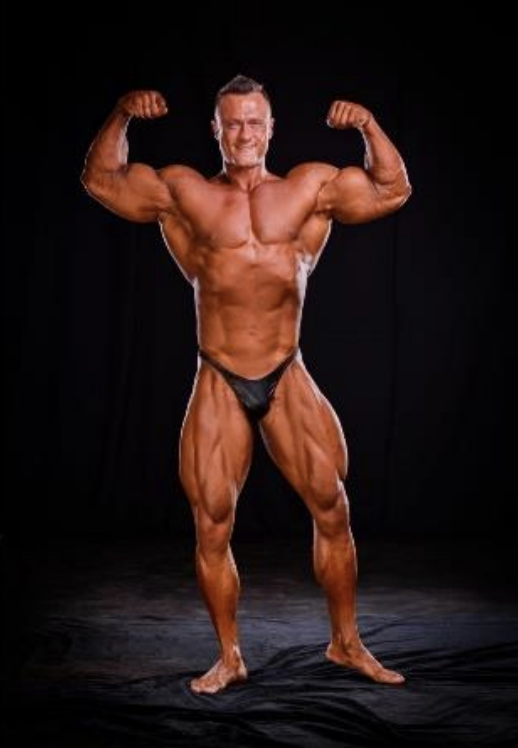
\includegraphics[width=0.75\linewidth, height=5cm]{figures/double_biceps.png}
            \caption{フロントダブルバイセップス}
            \label{fig:double_biceps}
        \end{minipage} &
        \begin{minipage}[t]{.33\textwidth}
            \centering
            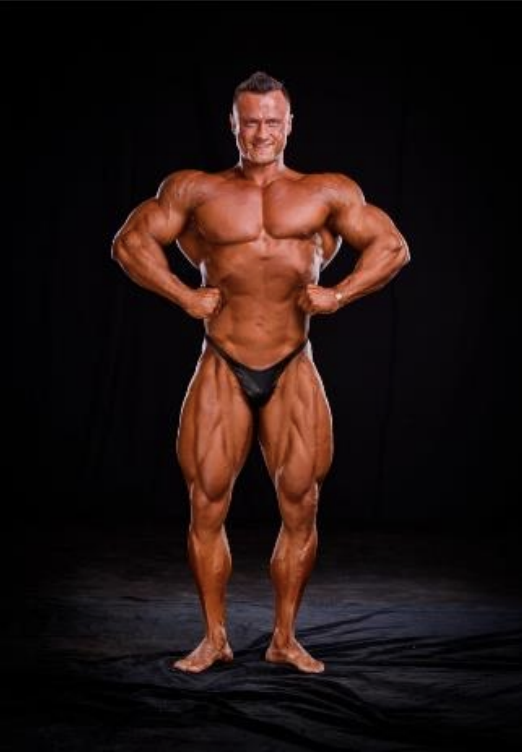
\includegraphics[width=0.75\linewidth, height=5cm]{figures/front_lat_spread.png}
            \caption{フロントラットスプレッド}
            \label{fig:front_lat_spread}
        \end{minipage} &
        \begin{minipage}[t]{.33\textwidth}
            \centering
            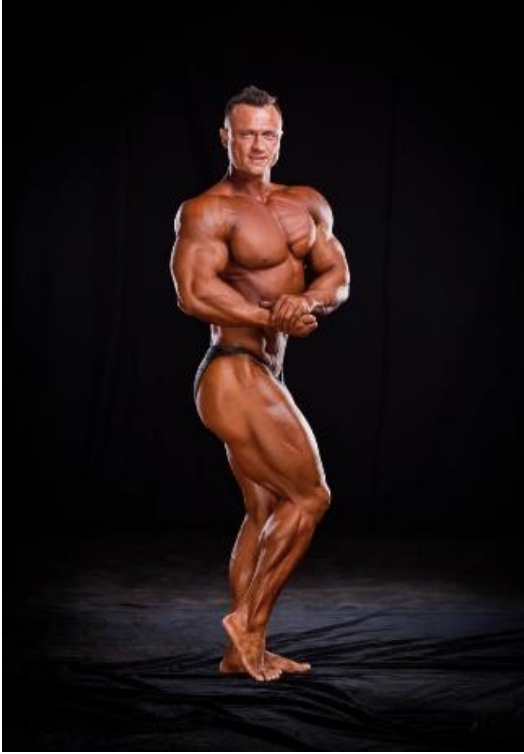
\includegraphics[width=0.75\linewidth, height=5cm]{figures/side_chest.png}
            \caption{サイドチェスト}
            \label{fig:side_chest}
        \end{minipage}
    \end{tabular}

    \begin{tabular}{cccc}
        \begin{minipage}{.25\textwidth}
            \centering
            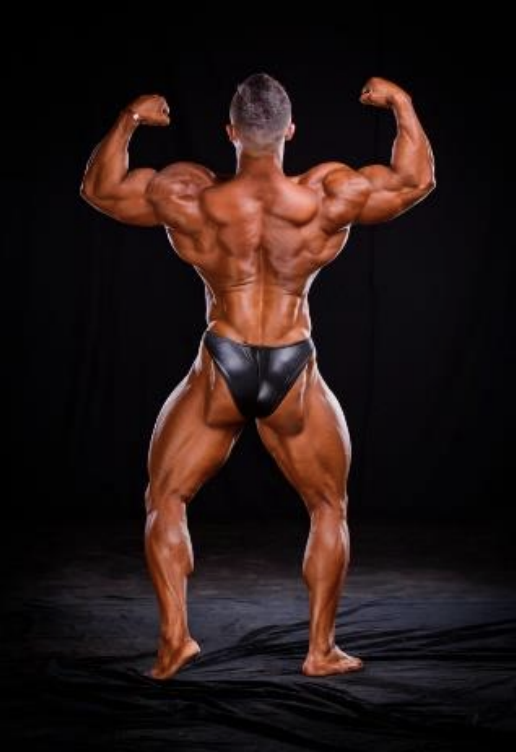
\includegraphics[width=0.75\linewidth, height=3.75cm]{figures/back_double_biceps.png}
            \caption{バックダブルバイセップス}
            \label{fig:back_double_biceps}
        \end{minipage} &
        \begin{minipage}{.25\textwidth}
            \centering
            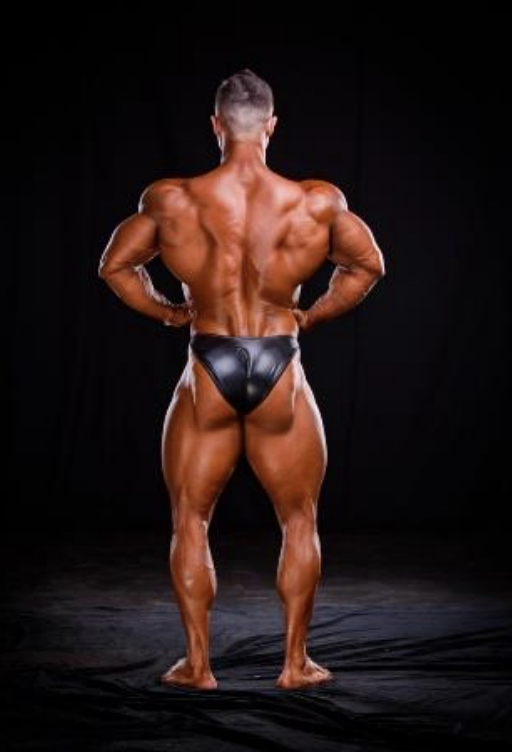
\includegraphics[width=0.75\linewidth, height=3.75cm]{figures/back_lat_spread.png}
            \caption{バックラットスプレッド}
            \label{fig:back_lat_spread}
        \end{minipage} &
        \begin{minipage}{.25\textwidth}
            \centering
            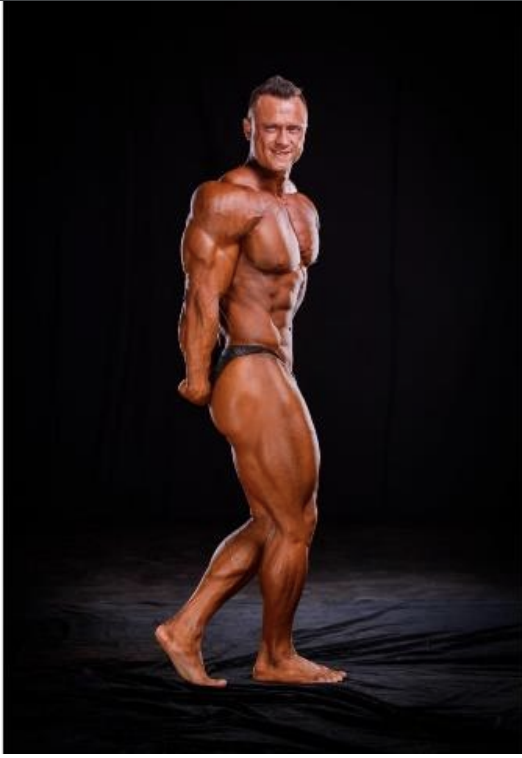
\includegraphics[width=0.75\linewidth, height=3.75cm]{figures/side_triceps.png}
            \caption{サイドトライセップス}
            \label{fig:side_triceps}
        \end{minipage} &
        \begin{minipage}{.25\textwidth}
            \centering
            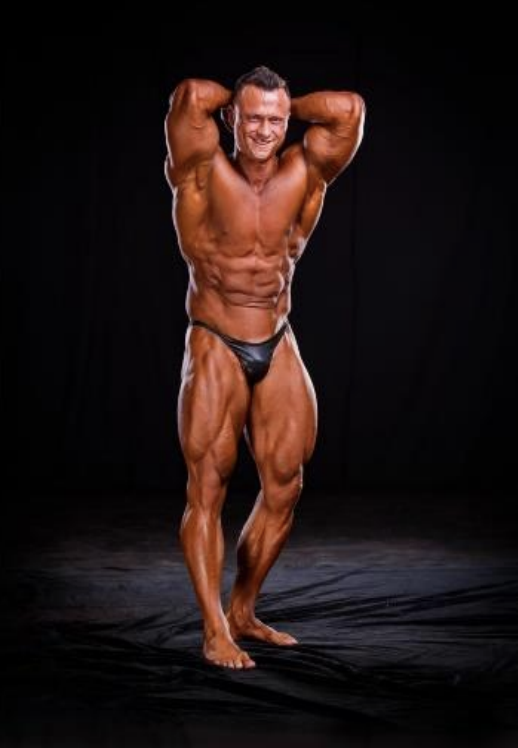
\includegraphics[width=0.75\linewidth, height=3.75cm]{figures/abdominal_and_sai.png}
            \caption{アブドミナルアンドサイ}
            \label{fig:abdominal_and_sai}
        \end{minipage}
    \end{tabular}
\end{figure}


\section{ボディビルにおけるポージングの重要性}
JBBFにおけるボディビルの具体的な審査のポイントはJBBF競技マニュアルのメンズボディビル審査ポイントで以下のように定められている\cite{JBBF2023}。

\begin{enumerate}
  \item 究極の筋肉美
  \item 各部位の筋肉量
  \item 各部位のボリューム
  \item 各部位の密度
  \item 仕上がりのハードさ
  \item 上半身下半身左右のバランス
  \item ポージングセンス
  \item フリーポーズでの芸術性・表現力
  \item コスチュームの着こなし・身だしなみ
\end{enumerate}
このように、ポージングセンスは複数ある審査基準の一つであるが、他の審査基準で挙げられている肉体の完成度を見る項目をよりよくはっきするためには大切である。
ポージングはボディビルにおいてステージ上でできる唯一の要素であり、ポージングによって弱点を隠すことや、逆に強みをより活かすこともできる。


\section{骨格推定}
骨格推定とは深層学習などを用いて人物のポーズを可視化できる手法であり、モーションキャプチャーなどの特別な機器を使用することなく,
画像、動画データ、又はカメラからの入力を用いて人間のポーズを可視化することができる。
カーネギーメロン大学(CMU)の Zhe Caoら が「Realtime Multi-Person pose estimation」\cite{openpose}の論文で発表した、OpenPoseが一つの例である。OpenPoseでは図\ref{fig:openpose}のように、人物の骨格を推定しリアルタイムに可視化することができる。


骨格推定はさまざまなスポーツへ利用されている。上智大学大学院の金子ら \cite{soccer_openpose}はOpenPoseを用いてサッカーのシュートフォームを取得し、体の傾き、軸足、腰の回転、フォロースルーを特長量として用い、習熟度ごとに分類を行った。
\begin{figure}[htbp]
    \begin{center}
        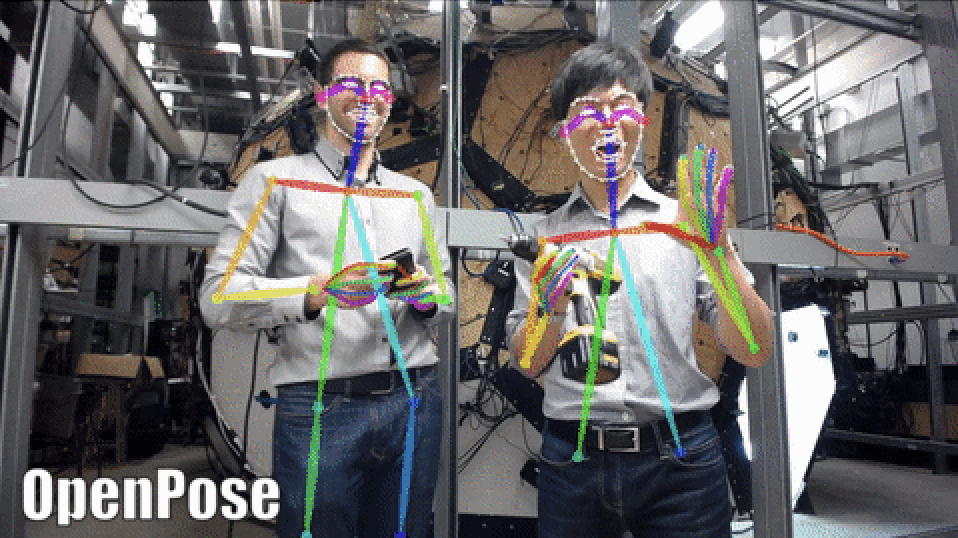
\includegraphics[width=7cm]{figures/openpose.png}
        \caption{OpenPose}
        \label{fig:openpose}
    \end{center}
  \end{figure}
\section{ガイダンス仮説}
ガイダンス仮説\cite{guidance_hypothesis}とは、フィードバックの頻度に関する仮説であり、学習中全ての試行においてフィードバックを与えると学習者はフィードバックに依存してしまい、
その結果、フィードバックを伴う練習中においてはパフォーマンスが優れているものの、フィードバックがない保持テストでは正確な運動を行えないことが多い。これは外在的フィードバックに依存してしまい、内在的フィードバックをおろそかにしてしまうためであると考えられている。
ここでいう内在的フィードバックとは、
私たちが動作を実行する際に自分の感覚に基づいてその動作を評価し、学習するプロセスである。
例えば、歩行時に足の裏から伝わる路面の感覚を認識することや、自分の進む方向を視覚的に確認することも、この内在的フィードバックの一例であることと言える。\cite{nagoyahml_feedback}

ガイダンス仮説提唱後、フィードバックの与え方については様々な研究がなされている。ガイダンス仮説の否定的な効果を軽減するために、フィードバックの頻度を減らすことでフィードバックへの依存を減らす方法が提案されている。
それ以外にも、フィードバックの回数をだんだんと減らしていく漸減式フィードバック(Faded feedback)\cite{Aoyagi2019}や複数の試行の平均のフィードバックを与える平均化フィードバック(Averaged feedback)\cite{Aoyagi2019}などがある。

\chapter{本研究における問題定義}
\label{issue}

\section{ボディビルにおけるポージングの重要性}
ポージングはトレーニングや減量と比べると練習時間が短く、相対的に重要度が下がってしまう傾向がある。
その原因としてはトレーニングの使用重量や減量における体重の変化のような定量的な指標がポージングには存在しないことが考えられる。
特に初心者では実際にステージで他の競技者と比較された経験が少ないため、ポージングの重要性を理解することが難しい。
また、ボディビルではトレーニングや、減量、日焼け、ポージングなどやることが多く、初心者は全てに時間やコストを払うのはとても大変である。
\section{ボディビルのポージングにおける悪いポージング}
ボディビルのポージングでは正解とされるポーズは存在しない。しかし、悪いポーズとされるポーズは存在する。
競技マニュアル\cite{JBBF2023}では悪いポーズの例として以下の図\ref{fig:badpose1},図\ref{fig:badpose2} が挙げられている。
図\ref{fig:badpose1}は片足を流していないことを指摘されていた。足を流すことでより足の筋肉のセパレーションやカットを強調できるため流していないことを指摘されていると考えられる。
図\ref{fig:badpose2}は腕をあげすぎていることを指摘されていた。腕をあげすぎてしまうと背中の広がりや上腕二頭筋などを強調することができないためこのような指摘がされたと考えられる。

  \begin{figure}[H]
    \begin{center}
        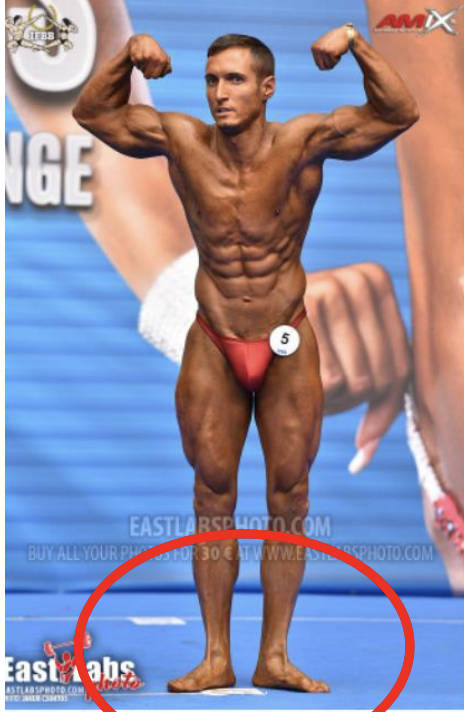
\includegraphics[width=7cm]{figures/badpose1.png}
        \caption{悪いポーズの例1}
        \label{fig:badpose1}
    \end{center}
  \end{figure}
  \begin{figure}[H]
    \begin{center}
        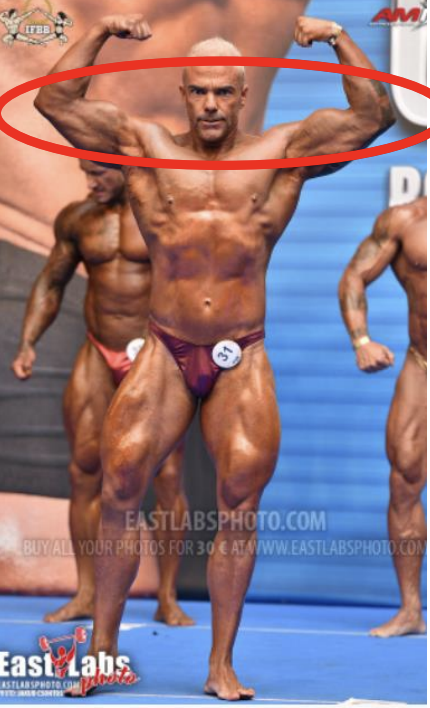
\includegraphics[width=7cm]{figures/badpose2.png}
        \caption{悪いポーズの例2}
        \label{fig:badpose2}
    \end{center}
  \end{figure}
\section{既存の練習方法における課題}
\subsection*{鏡を用いた練習}
ボディビルのポージング練習では鏡の前でポーズを取り、視覚的に確認しながらポーズを修正していく方法が一般的である。しかし、初心者では鏡を使った練習ではどこを修正したら良いかわかりづらい。
また、鏡を見ながらの練習では左右反転している状態や、視点が自分と同じ高さにあることなどを理由に実際のステージ下にいる審査員とは異なる見え方をするため、本番を意識したポーズを獲得することが難しい。
一般的な家庭にあるサイズの鏡ではポーズをとった時に全身が映らなかったり、全身を俯瞰して見ることが難しかったりといった問題がある。
\subsection*{動画や画像を使った練習}
写真や動画に撮る方法も鏡を使う練習と同じくよく行われる方法だ。カメラで撮影することで鏡と違い第三者視点でのポージングの確認ができることがメリットとして挙げられる。
第三者視点で見れることで、ポーズ全体を俯瞰して見ることや背中側のポーズを確認するといったことは可能になる。背中側のポーズは鏡では確認することが難しく、ポーズ習得の難易度が高いものになる。
しかしカメラで撮影する場合は、撮影のセッティングや撮影後の確認の手間がかかる。画像と比較してポーズを修正するには大きなディスプレイを利用するか、自身で覚えて鏡に映ったポーズと比較するといった方法が考えられるが、どちらも手間がかかる。
トップボディビルダーは毎トレーニング後にポージング練習を行うことを推奨していることが多いが、その度に撮影を行うのは鏡を使うことと比べ手軽とは言えない。
\subsection*{他者からの指導}
上記2つの練習方法はどちらも1人で行う場合ではあるが、ポーズ改善のために他者からフィードバックを受ける方法もポーズを獲得するために重要な要素だ。
その場合、指導を受ける相手としてボディビルの専門のトレーナーや、大会出場経験の豊富な競技者という選択肢がある。しかし、専門のトレーナーに指導を受ける場合は費用や時間の問題から初心者が何度も通うことはハードルが高い。
大会出場経験者の身の回りにいない場合は指導を受けることが難しい。

\section{仮説}
本研究では、次の仮説を検証する。
\begin{enumerate}
  \item 骨格推定用いた音声フィードバックを用いたポージング練習を行うことでポージングが改善される。
  \item 骨格推定用いた音声フィードバックを用いたポージング練習は鏡を用いたポージング練習と同等以上の効果を出すことができる。
\end{enumerate}
フィードバックがないことが初心者単独でのポージング練習の課題の一つとしてあがる。
骨格推定を用いたフィードバックに従いポーズを修正していくことでポーズが改善されると考えられる。
そして、他者を必要とせずフィードバックを与えることができれば、鏡を用いるポージング練習方法よりも骨格推定を用いたフィードバックを用いたポージング練習の方がポーズ獲得への効果が高いと考える。


\chapter{提案手法}
\label{proposed}
\section{提案}
\begin{itemize}
  \item ポーズ推定ライブラリであるMediaPipePose\cite{mediapipe_pose_landmarker}を用いて各関節の座標を取得する。その座標から関節角度を計測し、理想形との差異を測定する。
  \item 音声で大まかなフィードバックを与えることで利用者本人の内在的フィードバックによるポーズ習得をさせる。
\end{itemize}
関節の座標同士を繋げ、ボーンを推測し、隣り合うボーンの角度を計測する。その角度をそれぞれの関節でシステムに登録した理想の角度と比較し、差異を計測する。
それぞれの関節において理想の角度との差を計算し、その差が一番大きい関節に対して音声でフィードバックを与える。

\section{実装}
実装は図\ref{fig:system_figure}のように行った。
\begin{enumerate}
  \item webカメラでポーズを撮影
  \item MediaPipePoseを用いて各関節の座標を推測
  \item フィードバックとして読み上げる言葉をVOICEVOXに送信
  \item VOICRVOXで音声データを生成
  \item PCのスピーカーでユーザーへフィードバック
  \end{enumerate}

\begin{figure}[htbp]
  \begin{center}
      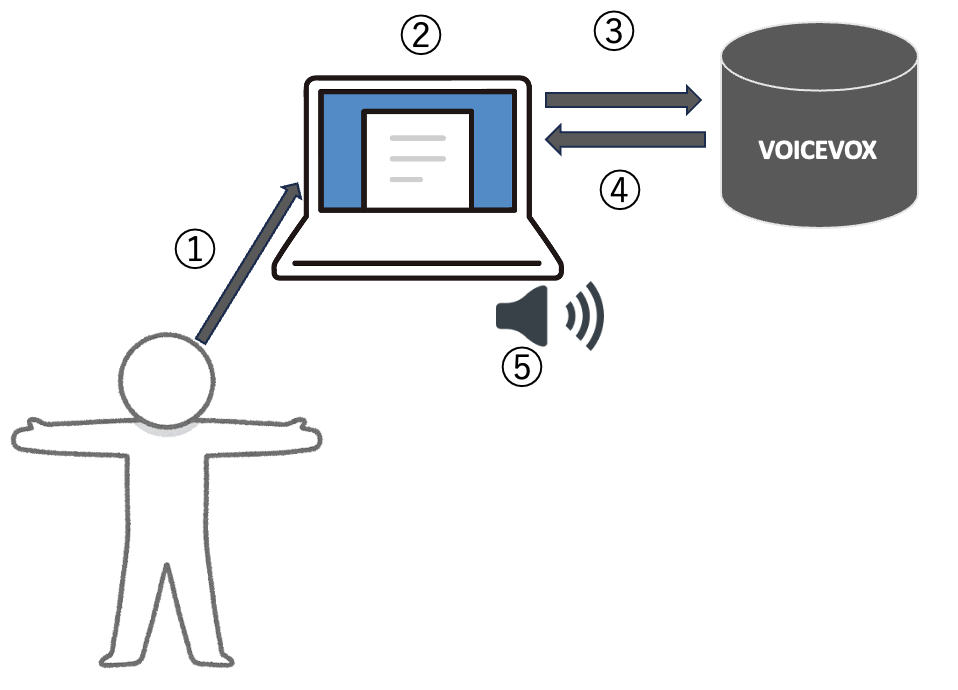
\includegraphics[width=7cm]{figures/system_figure.png}
      \caption{構成図}
      \label{fig:system_figure}
  \end{center}
\end{figure}


\chapter{実験}
\label{implementation}

\section{実験環境}
本実験では、理想的なボディビルのポーズを実現するために、特定の関節角度を有する3Dモデルを用いた。具体的には、ダブルバイセップスとクラシックポーズの2つのポーズを選定し、それぞれに対して3Dモデルを作成した。ダブルバイセップスのポーズでは、モデルの両肘は75度、両肩は160度に設定され、図\ref{fig:pose1}に示されている。一方、クラシックポーズでは、右肘が75度、左肘が180度、右肩が175度、左肩が165度に設定され、図\ref{fig:pose2}にて視覚化されている。

\begin{figure}[H]
\begin{center}
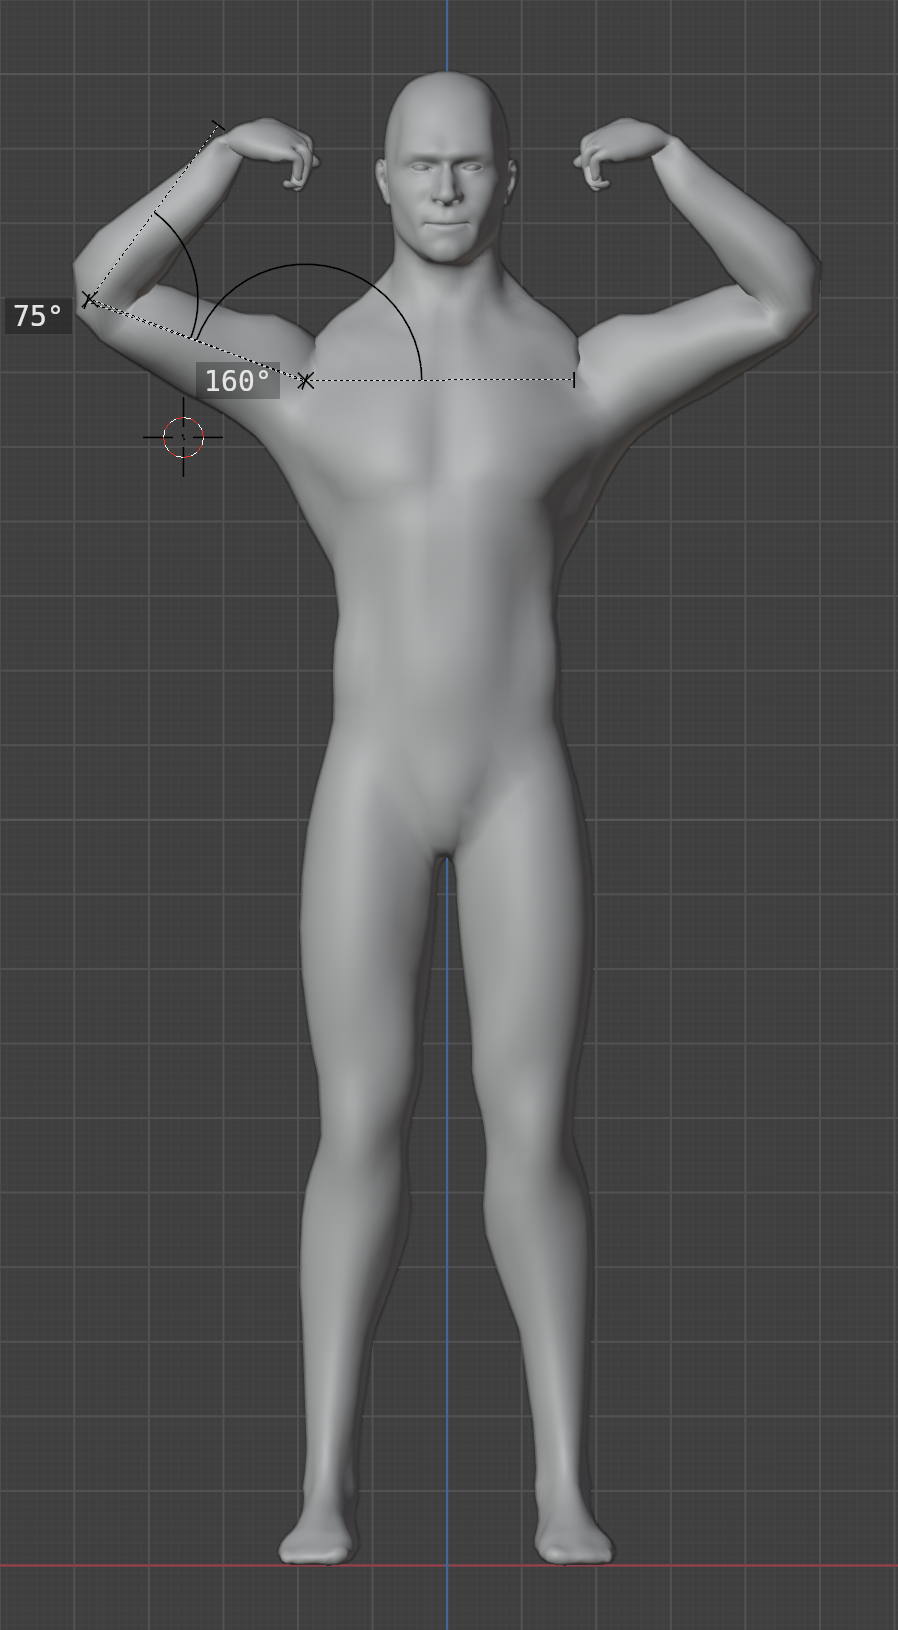
\includegraphics[width=6.5cm]{figures/pose1.png}
\caption{ダブルバイセップス(pose1)}
\label{fig:pose1}
\end{center}
\end{figure}
\begin{figure}[H]
\begin{center}
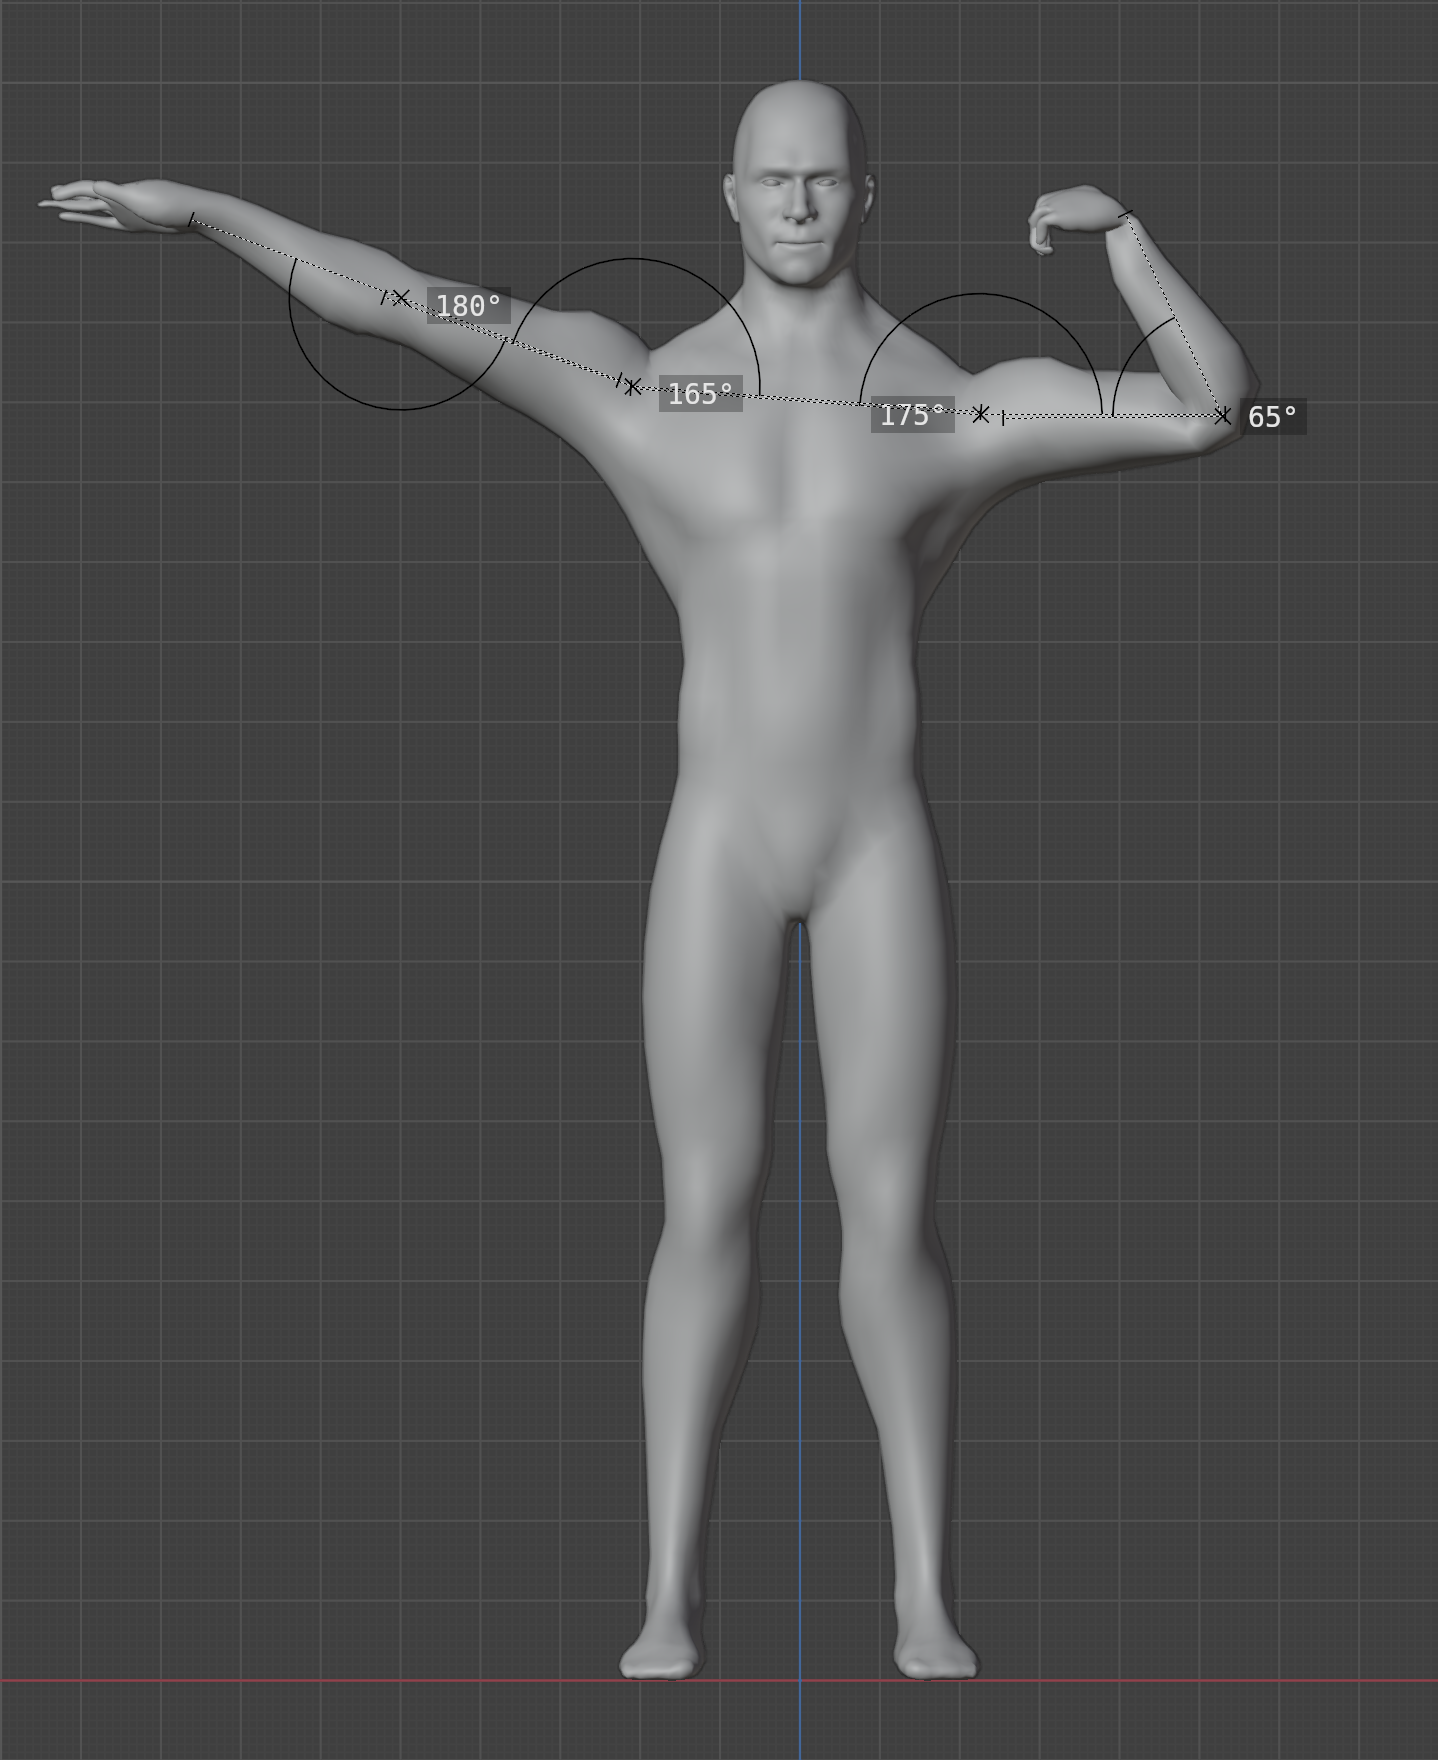
\includegraphics[width=6.5cm]{figures/pose2.png}
\caption{クラシックポーズ(pose2)}
\label{fig:pose2}
\end{center}
\end{figure}

被験者は2つのグループに分けられた。グループ1の被験者は、pose1を本実験で使用するシステムを利用して練習し、pose2は鏡を使用して練習した。対照的に、グループ2の被験者はpose1を鏡を用いて練習し、pose2は本システムを用いて練習することとした。

両グループの被験者には、システムを使用する練習と鏡を使用する練習をそれぞれ行ってもらい、各ポーズを30秒間保持すること、その後30秒間休憩することを1セットとし、合計10セットを完了させた。
システム、鏡どちらを使用して練習する場合でも理想のポーズとして図\ref{fig:pose1},図\ref{fig:pose2}を視認できる状態にた。
システム利用時にはシステムの音声に従ってポーズを修正するように指示し、鏡利用時には鏡の像と理想のポーズとしてみている図とを比較しポーズを修正するように指示をした。

被験者のポーズは練習前、練習後、練習から24時間後に計測した。図\ref{fig:schedule}

\begin{figure}[H]
\begin{center}
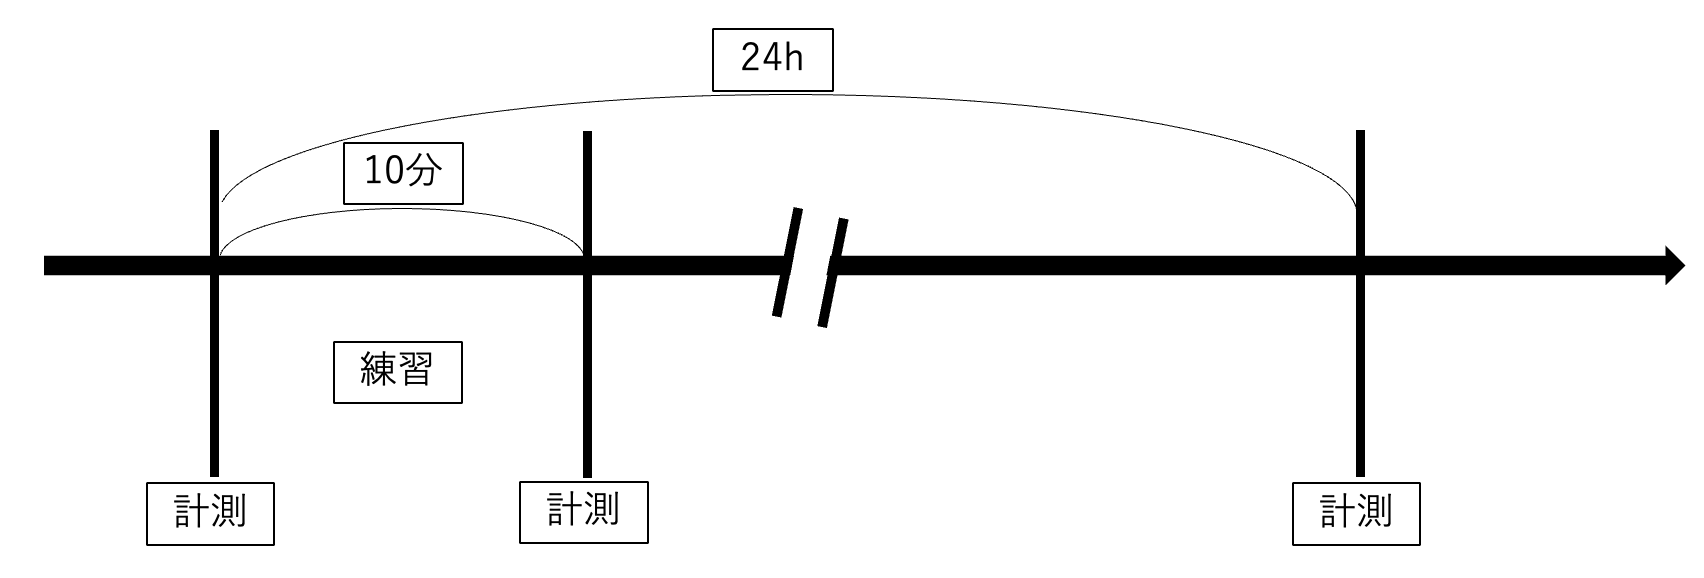
\includegraphics[width=9cm]{figures/schedule.png}
\caption{実験のスケジュール}
\label{fig:schedule}
\end{center}
\end{figure}
\chapter{評価}

\label{evaluation}
本研究では、本システムを利用することでポーズが改善できるかの検証、また、既存の練習方法である鏡を用いた練習との比較を行うため、
練習前と練習後、練習から24時間後のポーズの比較と、各ポーズにおけるシステム利用群と鏡利用群の比較を行った。
\section{評価内容}
  今回はシステムでのフィードバックでは両肘、両肩の角度についてフィードバックを行なっていたため、評価の際も同様に両肘、両肩の角度について評価を行った。


  肩の角度 \(\theta_{\text{肩}}\) は、上腕の単位ベクトル \(\vec{u}\) と両肩を結ぶ線の単位ベクトル \(\vec{w}\) を用いて計算することができる。この角度は、以下の式で定義される:

  \[
  \theta_{\text{肩}} = \cos\left( \frac{\vec{u} \cdot \vec{w}}{\|\vec{u}\| \|\vec{w}\|} \right) \times \frac{180}{\pi}
  \]


  同様に、肘の角度 \(\theta_{\text{肘}}\) は、前腕の単位ベクトル \(\vec{v}\) と上腕の単位ベクトル \(\vec{u}\) を使用して次のように計算される:

  \[
  \theta_{\text{肘}} = \cos\left( \frac{\vec{v} \cdot \vec{u}}{\|\vec{v}\| \|\vec{u}\|} \right) \times \frac{180}{\pi}
  \]

\section{測定方法}
  練習前、練習後、24時間後に写真を撮影し、それをMediapipe Poseを用い、ポーズを解析し角度を測定した。
  今回はMediapipe PoseでもBlazePose GHUM Heavyモデルを用いた。BlazePose GHUM Heavyモデルは表 \ref{tab:pose-estimation-quality} に示す通り同じBlazePose GHUMのモデルや、AlphaPose ResNet50、Apple Visionと比較しても様々なアクティビティにおいて精度が高いことが報告されている。
  この評価で用いられているPCK@0.2とは、人体の各部位の予測点と実際の点の距離が、人体の幅の20\%以内にあるかどうかを判定する指標である。\cite{PCK} また、利用者の属する地域別の精度は 図\ref{fig:Model-Accuracy-by-Race} に示す。今回の被験者の所属する日本は、Eastern Asiaに属するが、Eastern Asiaでの精度は今回利用するHeavyモデルではPDJという手法で92.6\%となっている。PDJはPCK@0.2と同義である。

  \begin{table}[ht]
    \centering
    \caption{様々なアクティビティにおける様々なモデルのPCK@0.2の比較 \cite{pose-estimation-quality}}
    \begin{tabular}{|l|c|c|c|}
    \hline
    \textbf{Method} & \textbf{Yoga} & \textbf{Dance} & \textbf{HIIT} \\
                    & PCK@0.2       & PCK@0.2        & PCK@0.2       \\ 
    \hline
    BlazePose GHUM Heavy                                                      & \textbf{96.4} & \textbf{97.2} & \textbf{97.5} \\
    BlazePose GHUM Full                                                       & \textbf{95.5} & \textbf{96.3} & \textbf{95.7} \\
    BlazePose GHUM Lite                                                       & \textbf{90.2} & \textbf{92.5} & \textbf{93.5} \\
    \href{https://github.com/MVIG-SJTU/AlphaPose}{AlphaPose ResNet50}         & \textbf{96.0} & \textbf{95.5} & \textbf{96.0} \\
    \href{https://developer.apple.com/documentation/vision/detecting_human_body_poses_in_images}{Apple Vision} & \textbf{82.7} & \textbf{91.4} & \textbf{88.6} \\
    \hline
    \end{tabular}
    \label{tab:pose-estimation-quality}
  \end{table}
    
  \begin{figure}[H]
    \begin{center}
    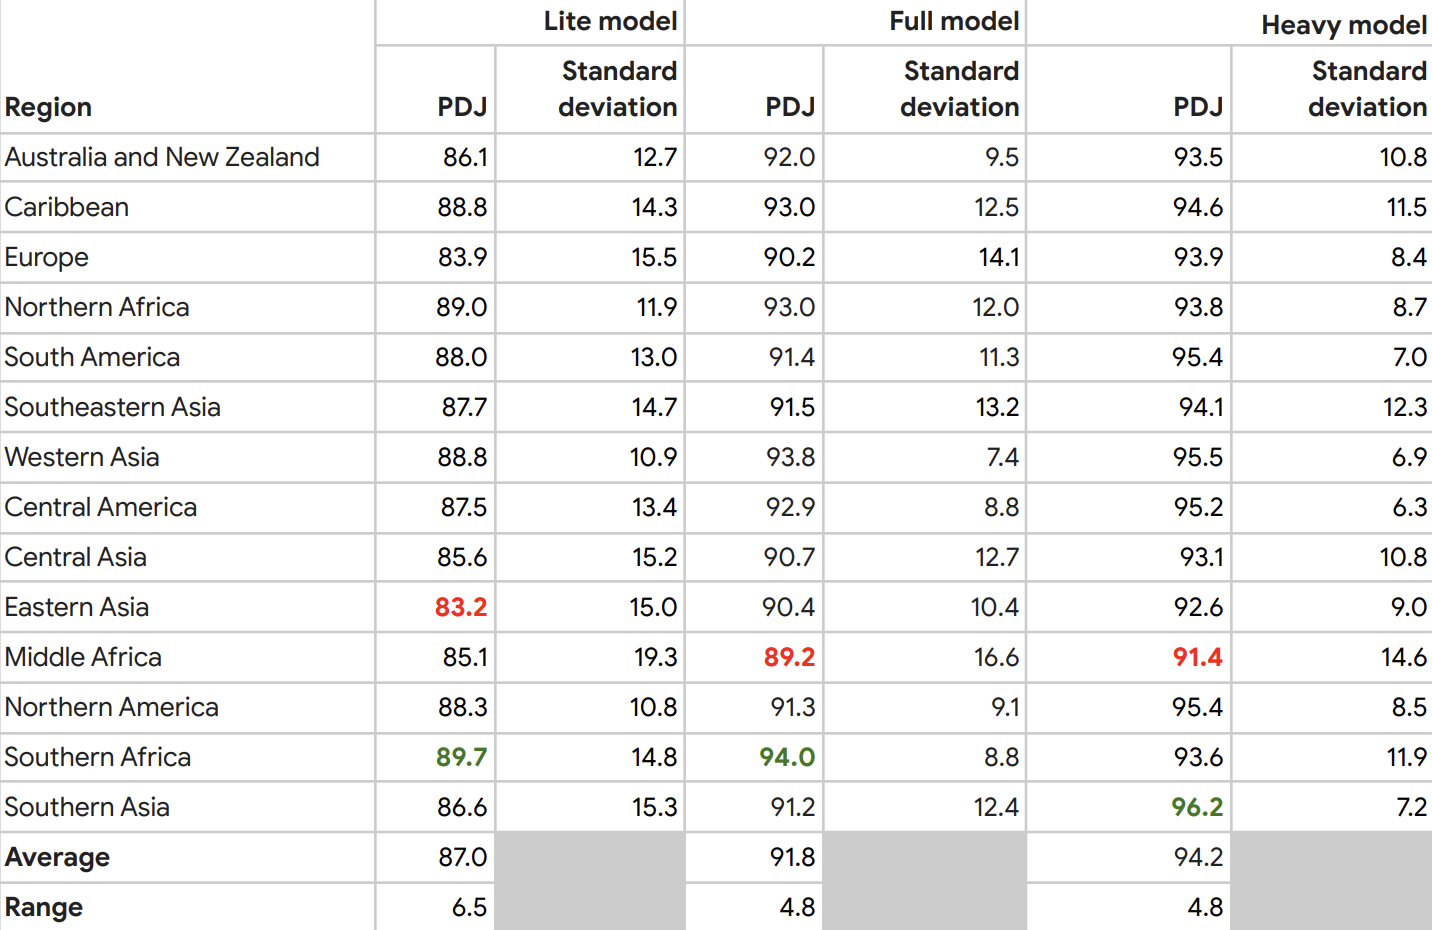
\includegraphics[width=12cm]{figures/Model_Accuracy_by_Race.png}
    \caption{様々な骨格推定モデルの地域別精度 \cite{Model-Accuracy-by-Race}}
    \label{fig:Model-Accuracy-by-Race}
    \end{center}
  \end{figure}

\section{検定手法}
  本研究の実験では被験者が少ないため、ノンパラメトリック検定を用いて検定を行った。
  同一被験者の練習後、24時間後と練習前の理想のポーズの角度の差の検定は、ウィルコクソンの符号付き順位和検定を用いた。
  また、システム利用群と鏡利用群の比較は、ウィルコクソンの順位和検定を用いた。有意水準は0.05とした。
\section{結果}
  本研究では練習で改善されたかどうかを評価したいため、練習前、練習後、24時間後のポーズの角度と理想とするポーズ(システムとしてさせたいポーズ)の両肘両肩の角度の差の平均 \(\bar{\theta}_{\text{angle\_dif}}\)を利用して評価する。
  それぞれの関節を右肘(RE)、左肘(LE)、右肩(RS)、左肩(LS)とし、以下のように定義した。

  \[
    \bar{\theta}_{\text{angle\_dif}} = \frac{1}{4} \sum_{i \in \{\text{RE, LE, RS, LS}\}} |\theta_{i, \text{Actual}} - \theta_{i, \text{Ideal}}|
  \]

  \subsection{練習前後、24時間後の比較}
    ここではシステムを利用して練習した群と鏡を利用して練習した群それぞれの練習前後、24時間後のポーズの理想の角度との差の結果を示す。
    \subsubsection{システム利用群の比較}
      図\ref{fig:pose1_system}にpose1に対してシステムを利用した群の練習前後、24時間後の結果と理想の角度との差の平均\(\bar{\theta}_{\text{angle\_dif}}\)の推移を示す。


      7名のうち、5名の被験者が練習直後は練習前よりポーズが改善されていることがわかる。しかしながら、24時間後では練習前より改善されている被験者は1名のみであった。
      検定の結果では練習後と練習前の差は有意性を示すことができず(p=0.8782)、24時間後と練習前の差も統計的に有意性を示すことができなかった(p=0.4674)。表\ref{table:pose1_system_p_value}

      \begin{figure}[H]
        \begin{center}
        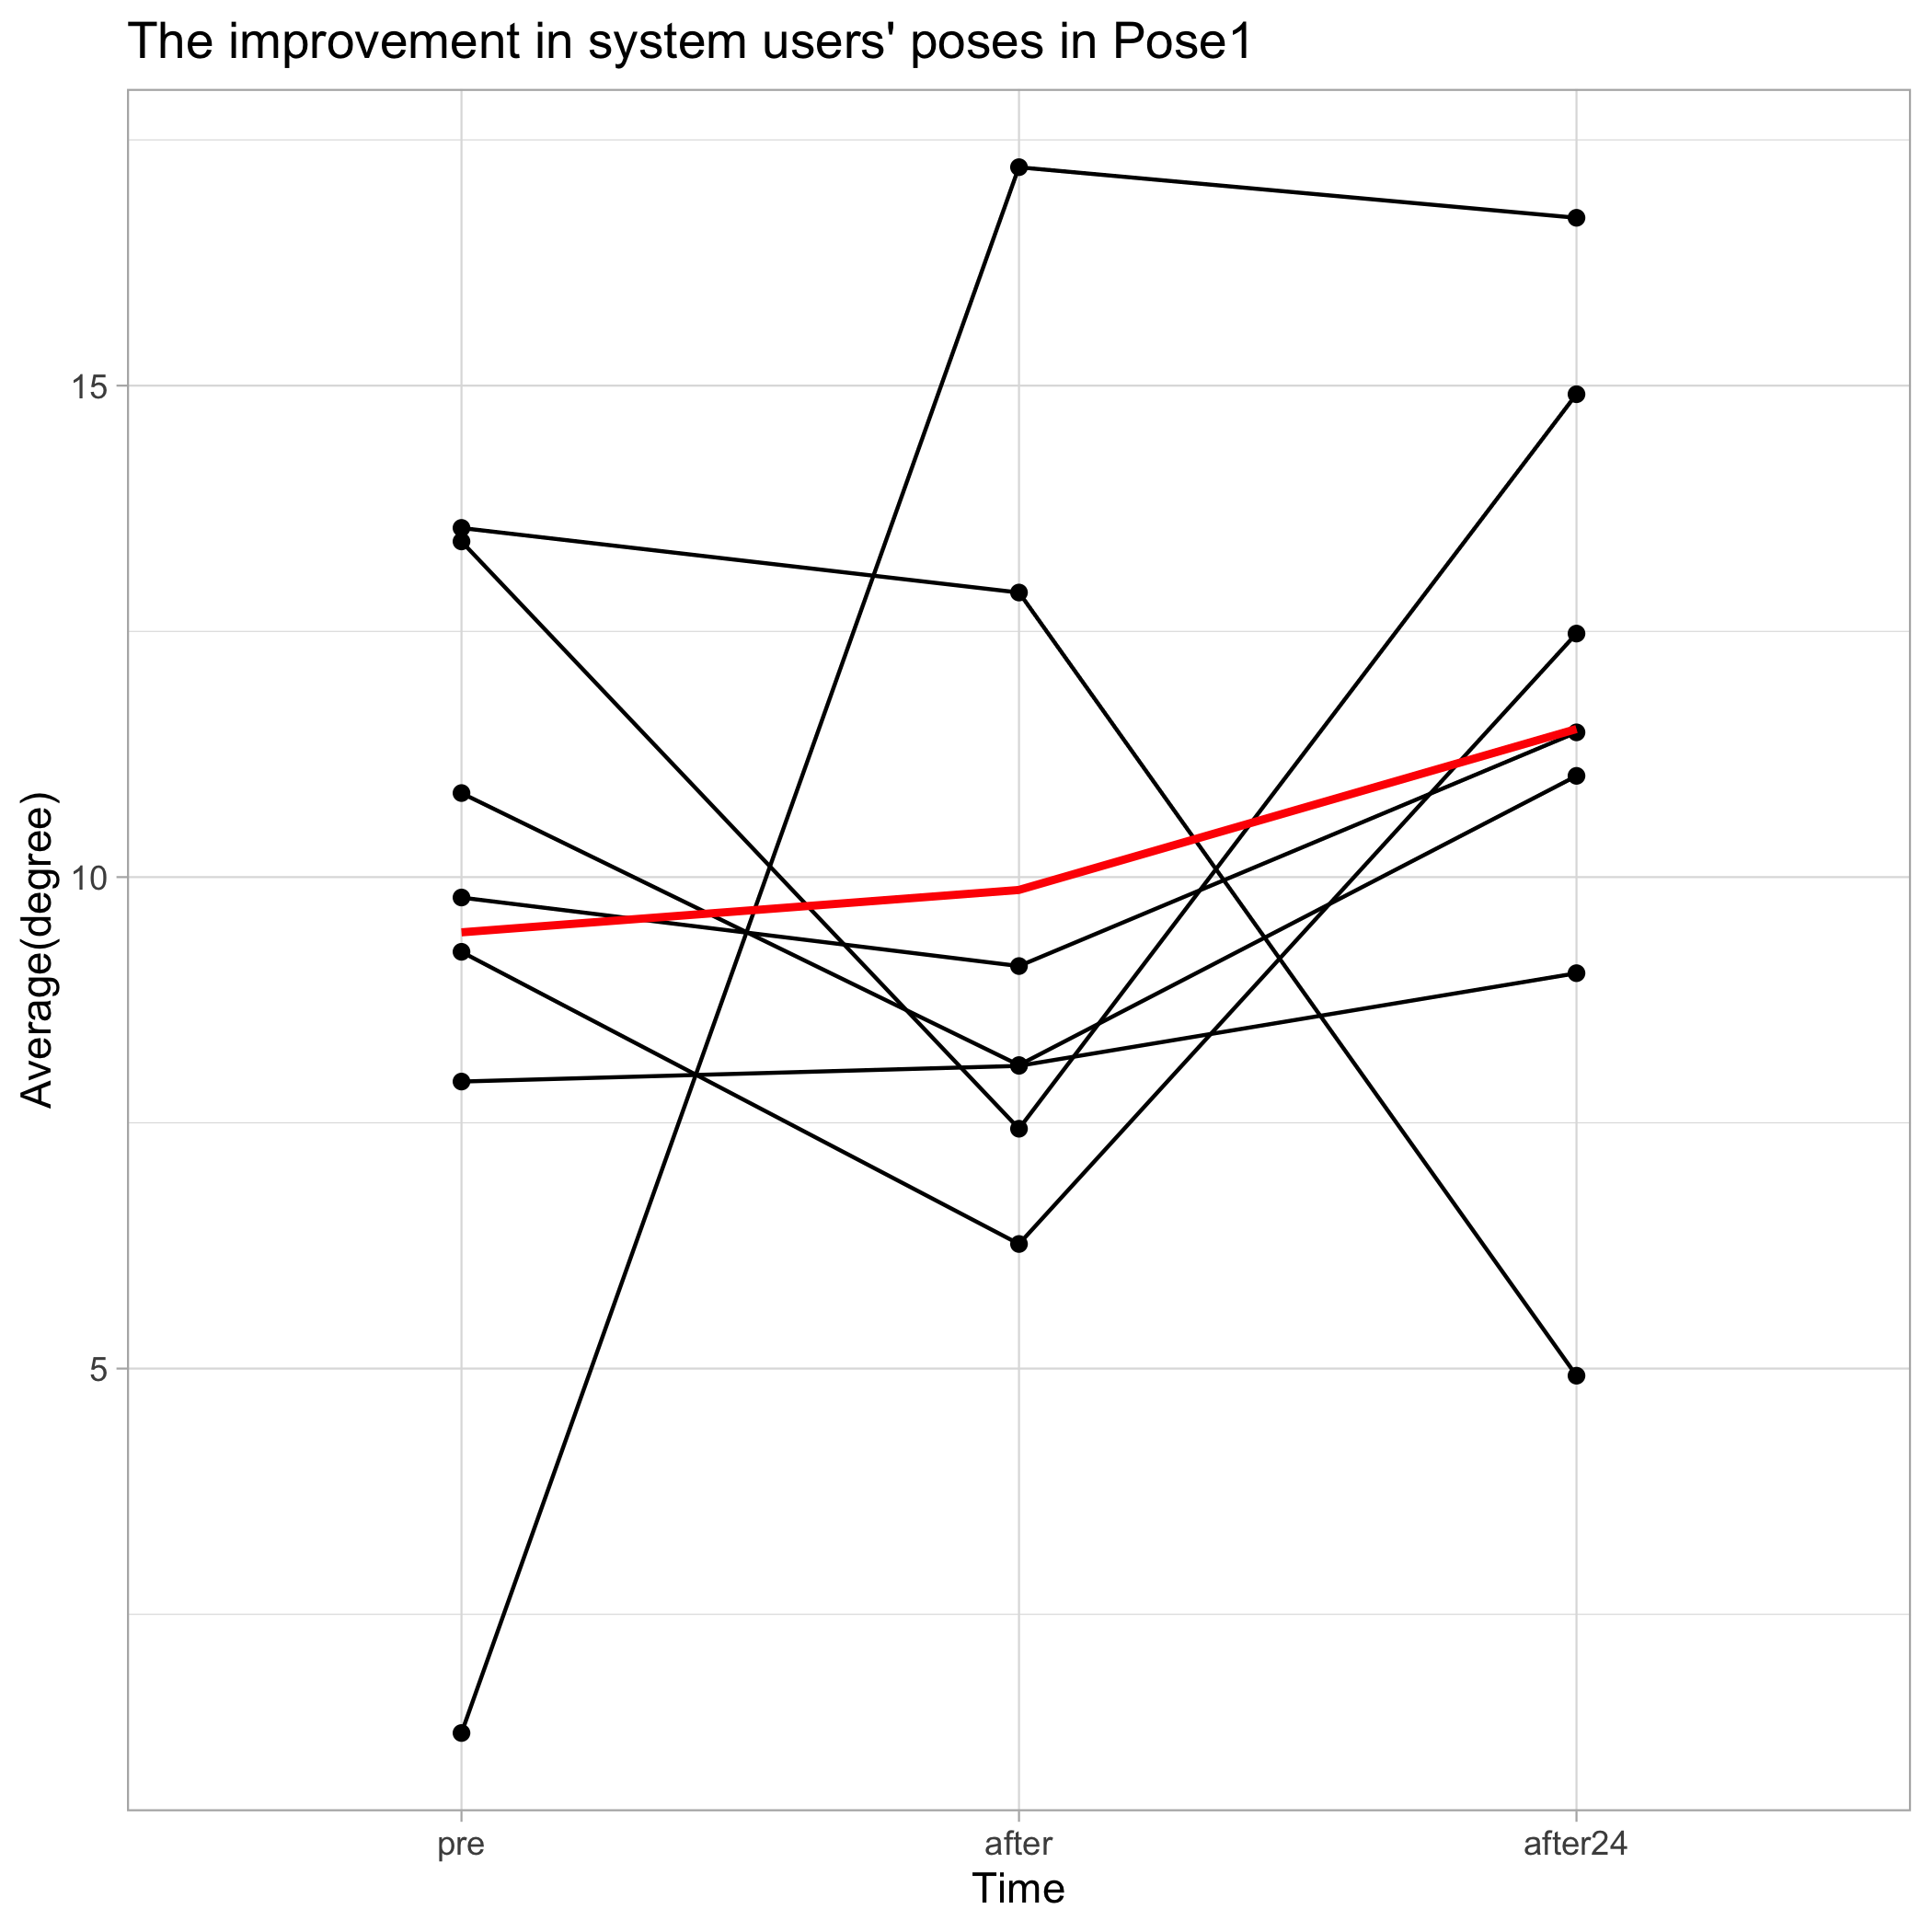
\includegraphics[width=9cm]{figures/pose1_system_true_graph.png}
        \caption{システム利用群のpose1の結果}
        \label{fig:pose1_system}
        \end{center}
      \end{figure}

      \begin{table}[h]
        \centering
        \caption{pose1における練習後、練習から24時間後と練習前の比較}
        \begin{tabular}{lcr}
        \hline
        \textbf{比較対象} & \textbf{p-value} & \textbf{MD} \\ \hline
        練習後-練習前 & 0.8782 & 0.4314286 \\ \hline
        24時間後-練習前 & 0.4674 & 2.068929 \\ \hline
        \end{tabular}
        \label{table:pose1_system_p_value}
        \end{table}

        図\ref{fig:pose2_system}にpose2に対してシステムを利用した群の練習前後、24時間後の結果と理想の角度との差の平均\(\bar{\theta}_{\text{angle\_dif}}\)の推移を示す。


      7名のうち、5名の被験者が練習直後は練習前よりポーズが改善されていることがわかる。しかしながら、24時間後では練習前より改善されている被験者は3名のみであった。
      検定の結果では練習後と練習前の差は有意性を示すことができず(p=0.07812)、24時間後と練習前の差も統計的に有意性を示すことができなかった(p=0.8125)。表\ref{table:pose2_system_p_value}
      \begin{figure}[H]
        \begin{center}
        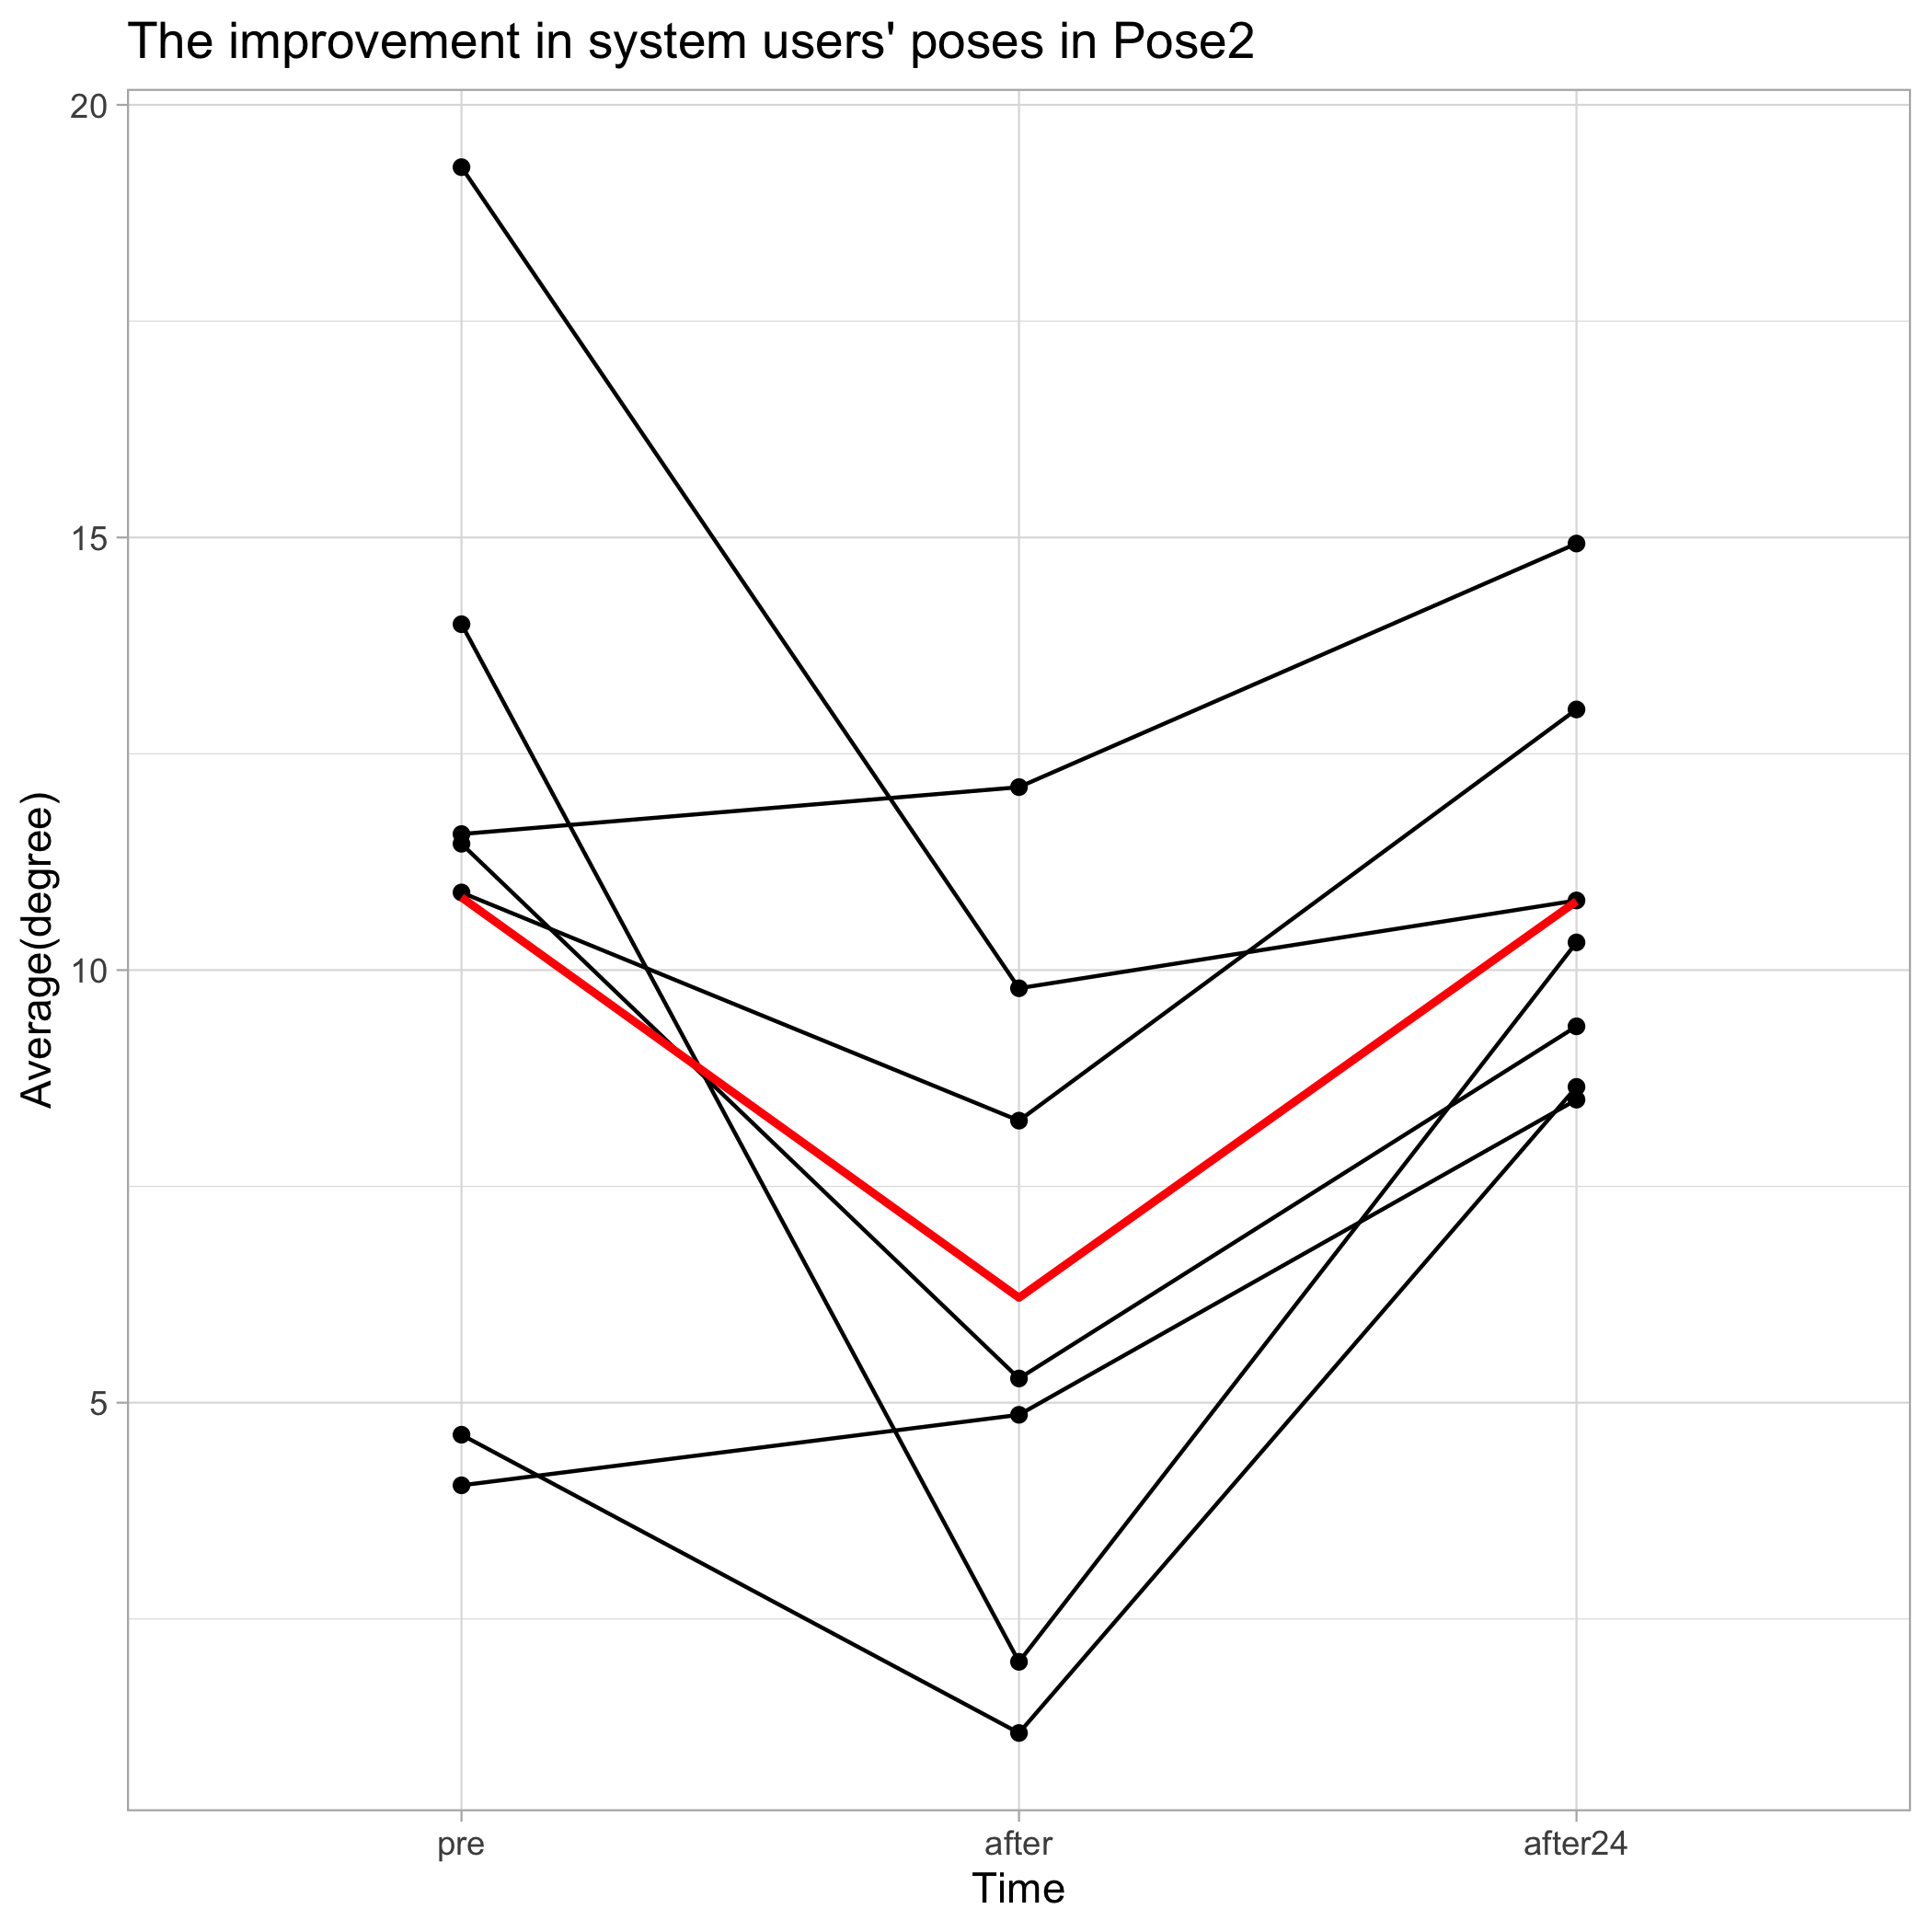
\includegraphics[width=9cm]{figures/pose2_system_true_graph.png}
        \caption{システム利用群のpose2の結果}
        \label{fig:pose2_system}
        \end{center}
      \end{figure}

      \begin{table}[ht]
        \centering
        \caption{pose2における練習後、練習から24時間後と練習前の比較}
        \begin{tabular}{lcr}
        \hline
        \textbf{比較対象} & \textbf{p-value} & \textbf{MD} \\ \hline
        after-pre & 0.07812 & -4.627143 \\ \hline
        after24-pre & 0.8125 & -0.04464286 \\ \hline
        \end{tabular}
        \label{table:pose2_system_p_value}
        \end{table}
    % ~~~~~~~~~~~~~~~~~~~~~~~~~~~~~~~~~~~~~~~~~~~~
    \subsubsection{鏡利用群の比較}
      図\ref{fig:pose1_mirror}にpose1に対して鏡を利用した群の練習前後、24時間後の結果と理想の角度との差の平均\(\bar{\theta}_{\text{angle\_dif}}\)を示す。


      7名のうち、5名の被験者が練習直後は練習前よりポーズが改善されていることがわかる。しかしながら、24時間後では練習前より改善されている被験者は4名であった。
      検定の結果では練習後と練習前の差は有意性を示すことができず(p=0.4688)、24時間後と練習前の差も統計的に有意性を示すことができなかった(p=0.5781)。表\ref{table:pose1_mirror_p_value}

      \begin{figure}[H]
        \begin{center}
        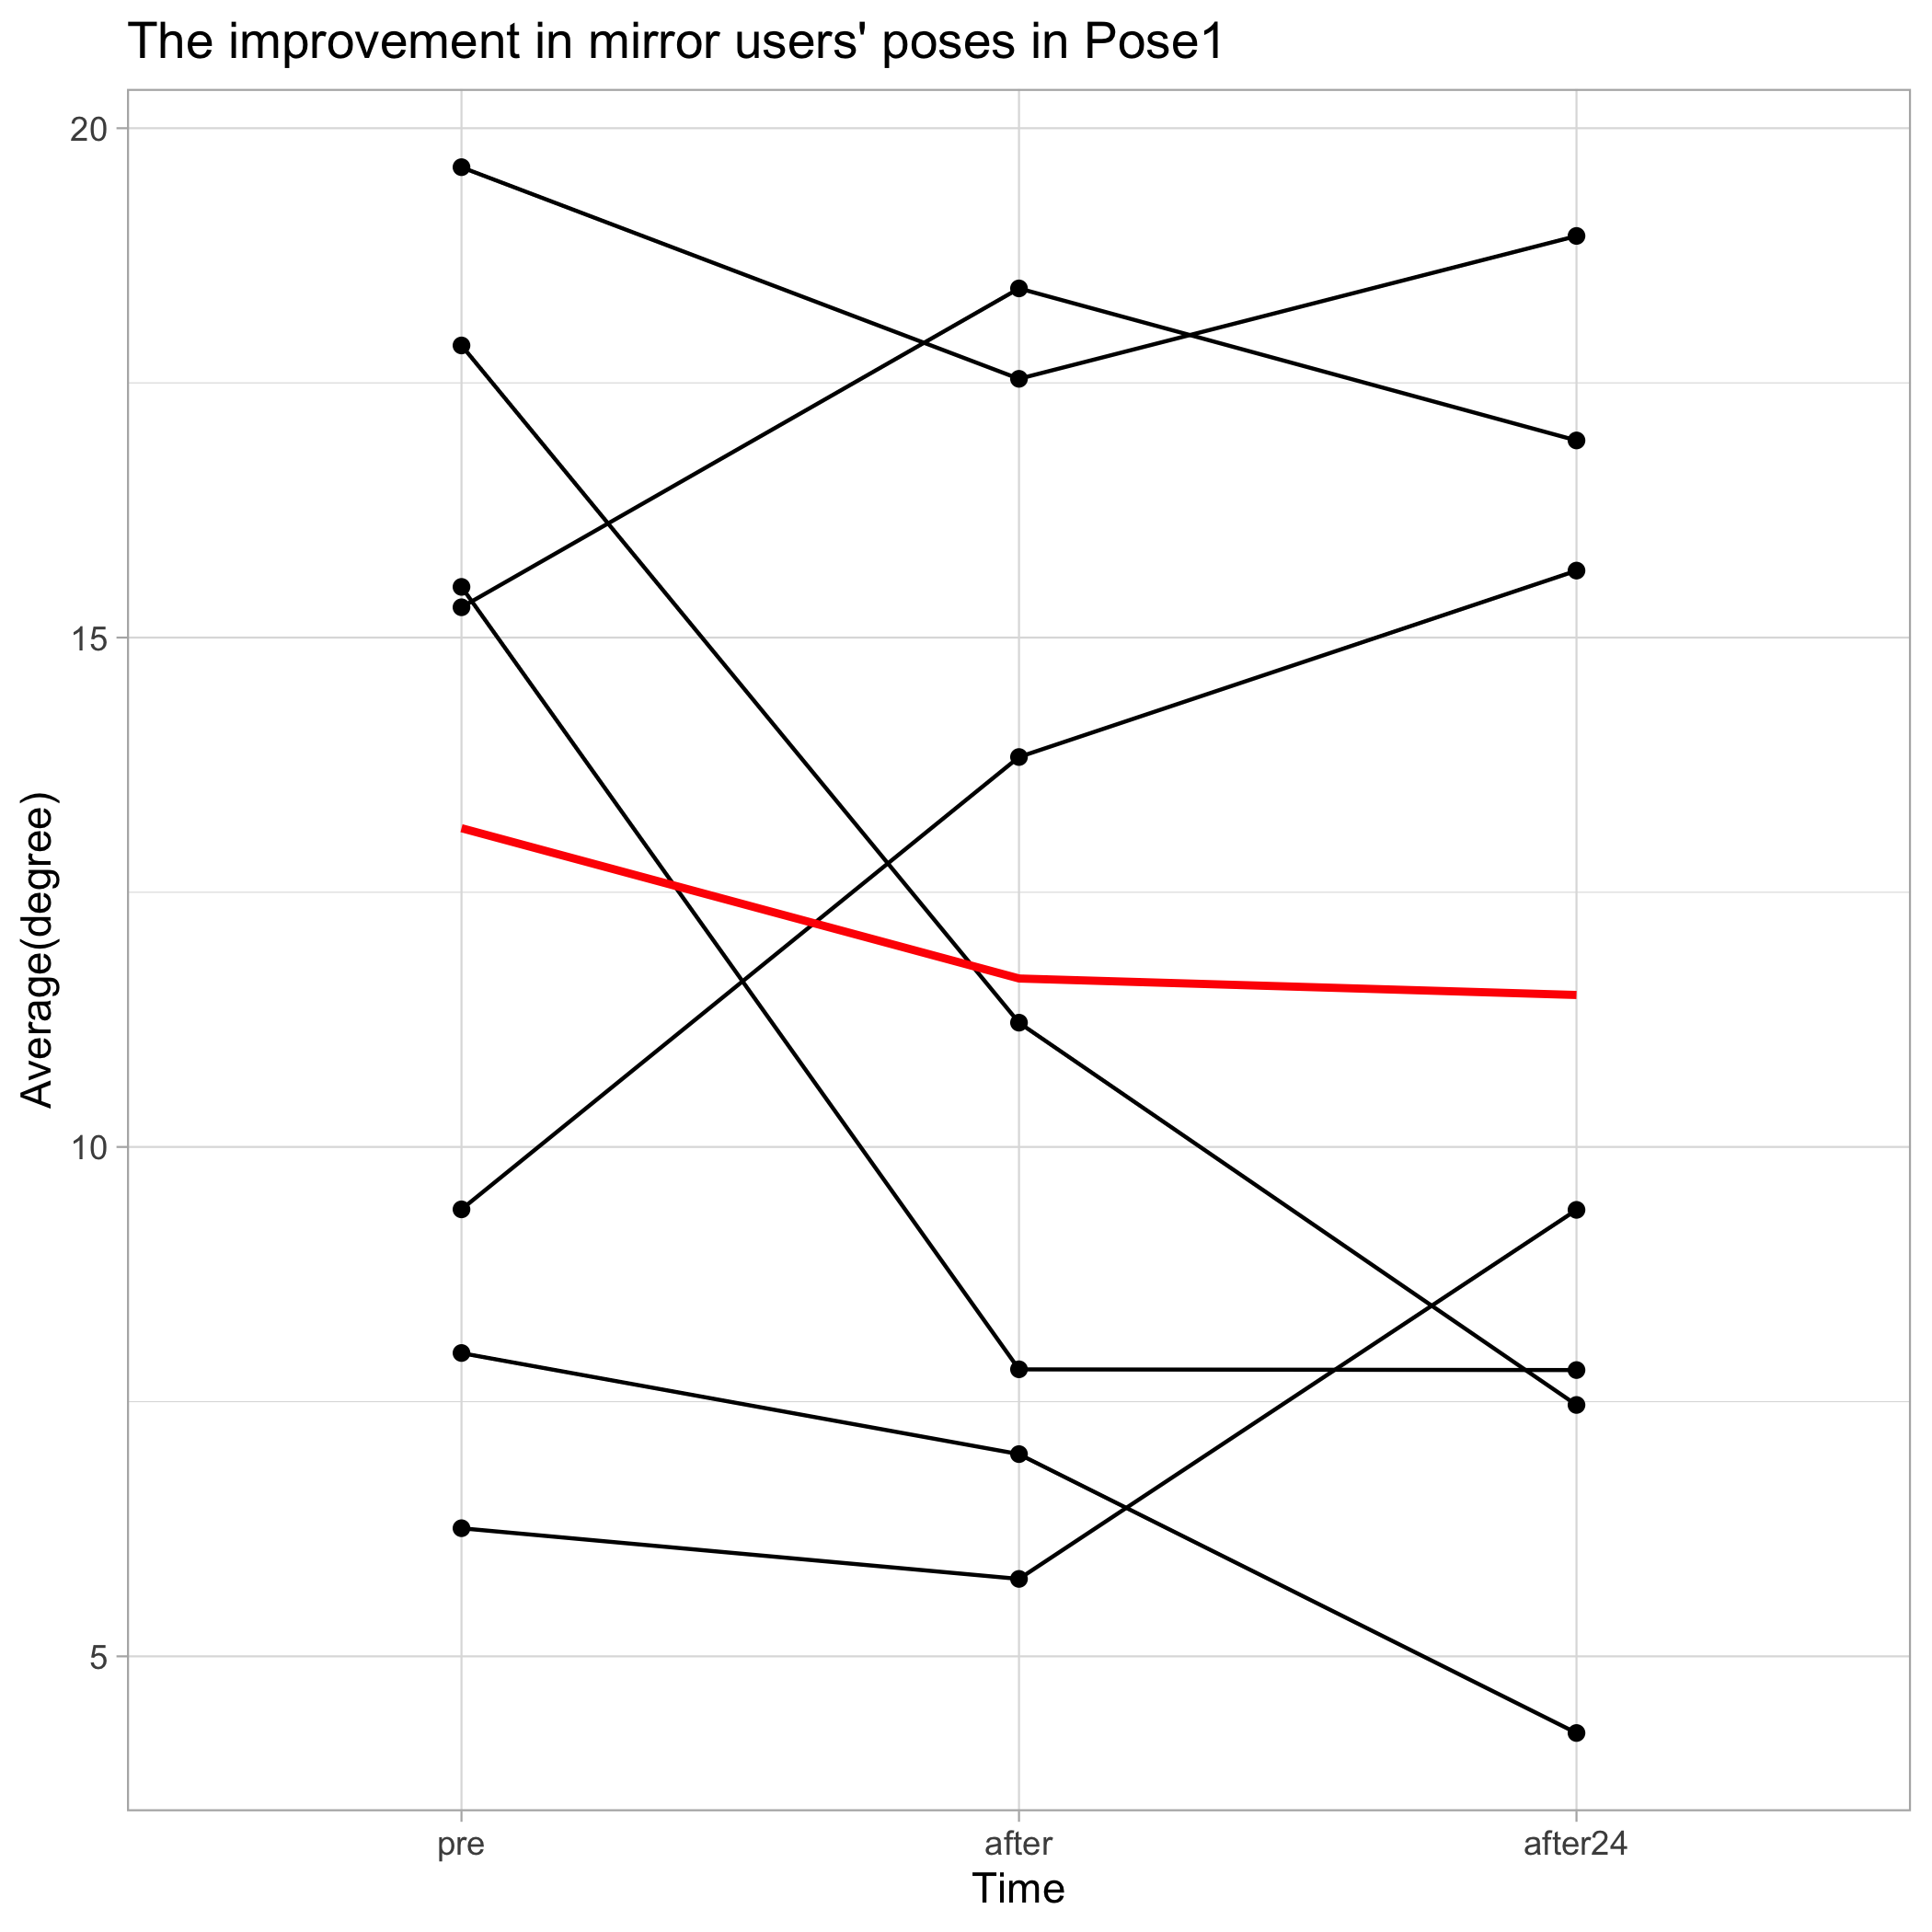
\includegraphics[width=9cm]{figures/pose1_system_false_graph.png}
        \caption{鏡利用群のpose1の結果}
        \label{fig:pose1_mirror}
        \end{center}
      \end{figure}

      \begin{table}[ht]
        \centering
        \caption{pose1における練習後、練習から24時間後と練習前の比較}
        \begin{tabular}{lcr}
        \hline
        \textbf{比較対象} & \textbf{p-value} & \textbf{MD} \\ \hline
        練習後-練習前 & 0.4688 & -1.475 \\ \hline
        24時間後-練習前 & 0.5781 & -1.637143 \\ \hline
        \end{tabular}
        \label{table:pose1_mirror_p_value}
        \end{table}

        図\ref{fig:pose2_mirror}にpose2に対して鏡を利用した群の練習前後、24時間後の結果と理想の角度との差の平均\(\bar{\theta}_{\text{angle\_dif}}\)を示す。


      7名のうち、6名の被験者が練習直後は練習前よりポーズが改善されていることがわかる。24時間後では練習前より改善されている被験者は3名であった。
      検定の結果では{\bf 練習後と練習前の差は有意であり、鏡の練習によって効果があったと考えられる(p=0.04688)}。 一方で、24時間後と練習前の差は統計的に有意性を示すことができなかった(p=0.8125)。表\ref{table:pose2_mirror_p_value}
      \begin{figure}[H]
        \begin{center}
        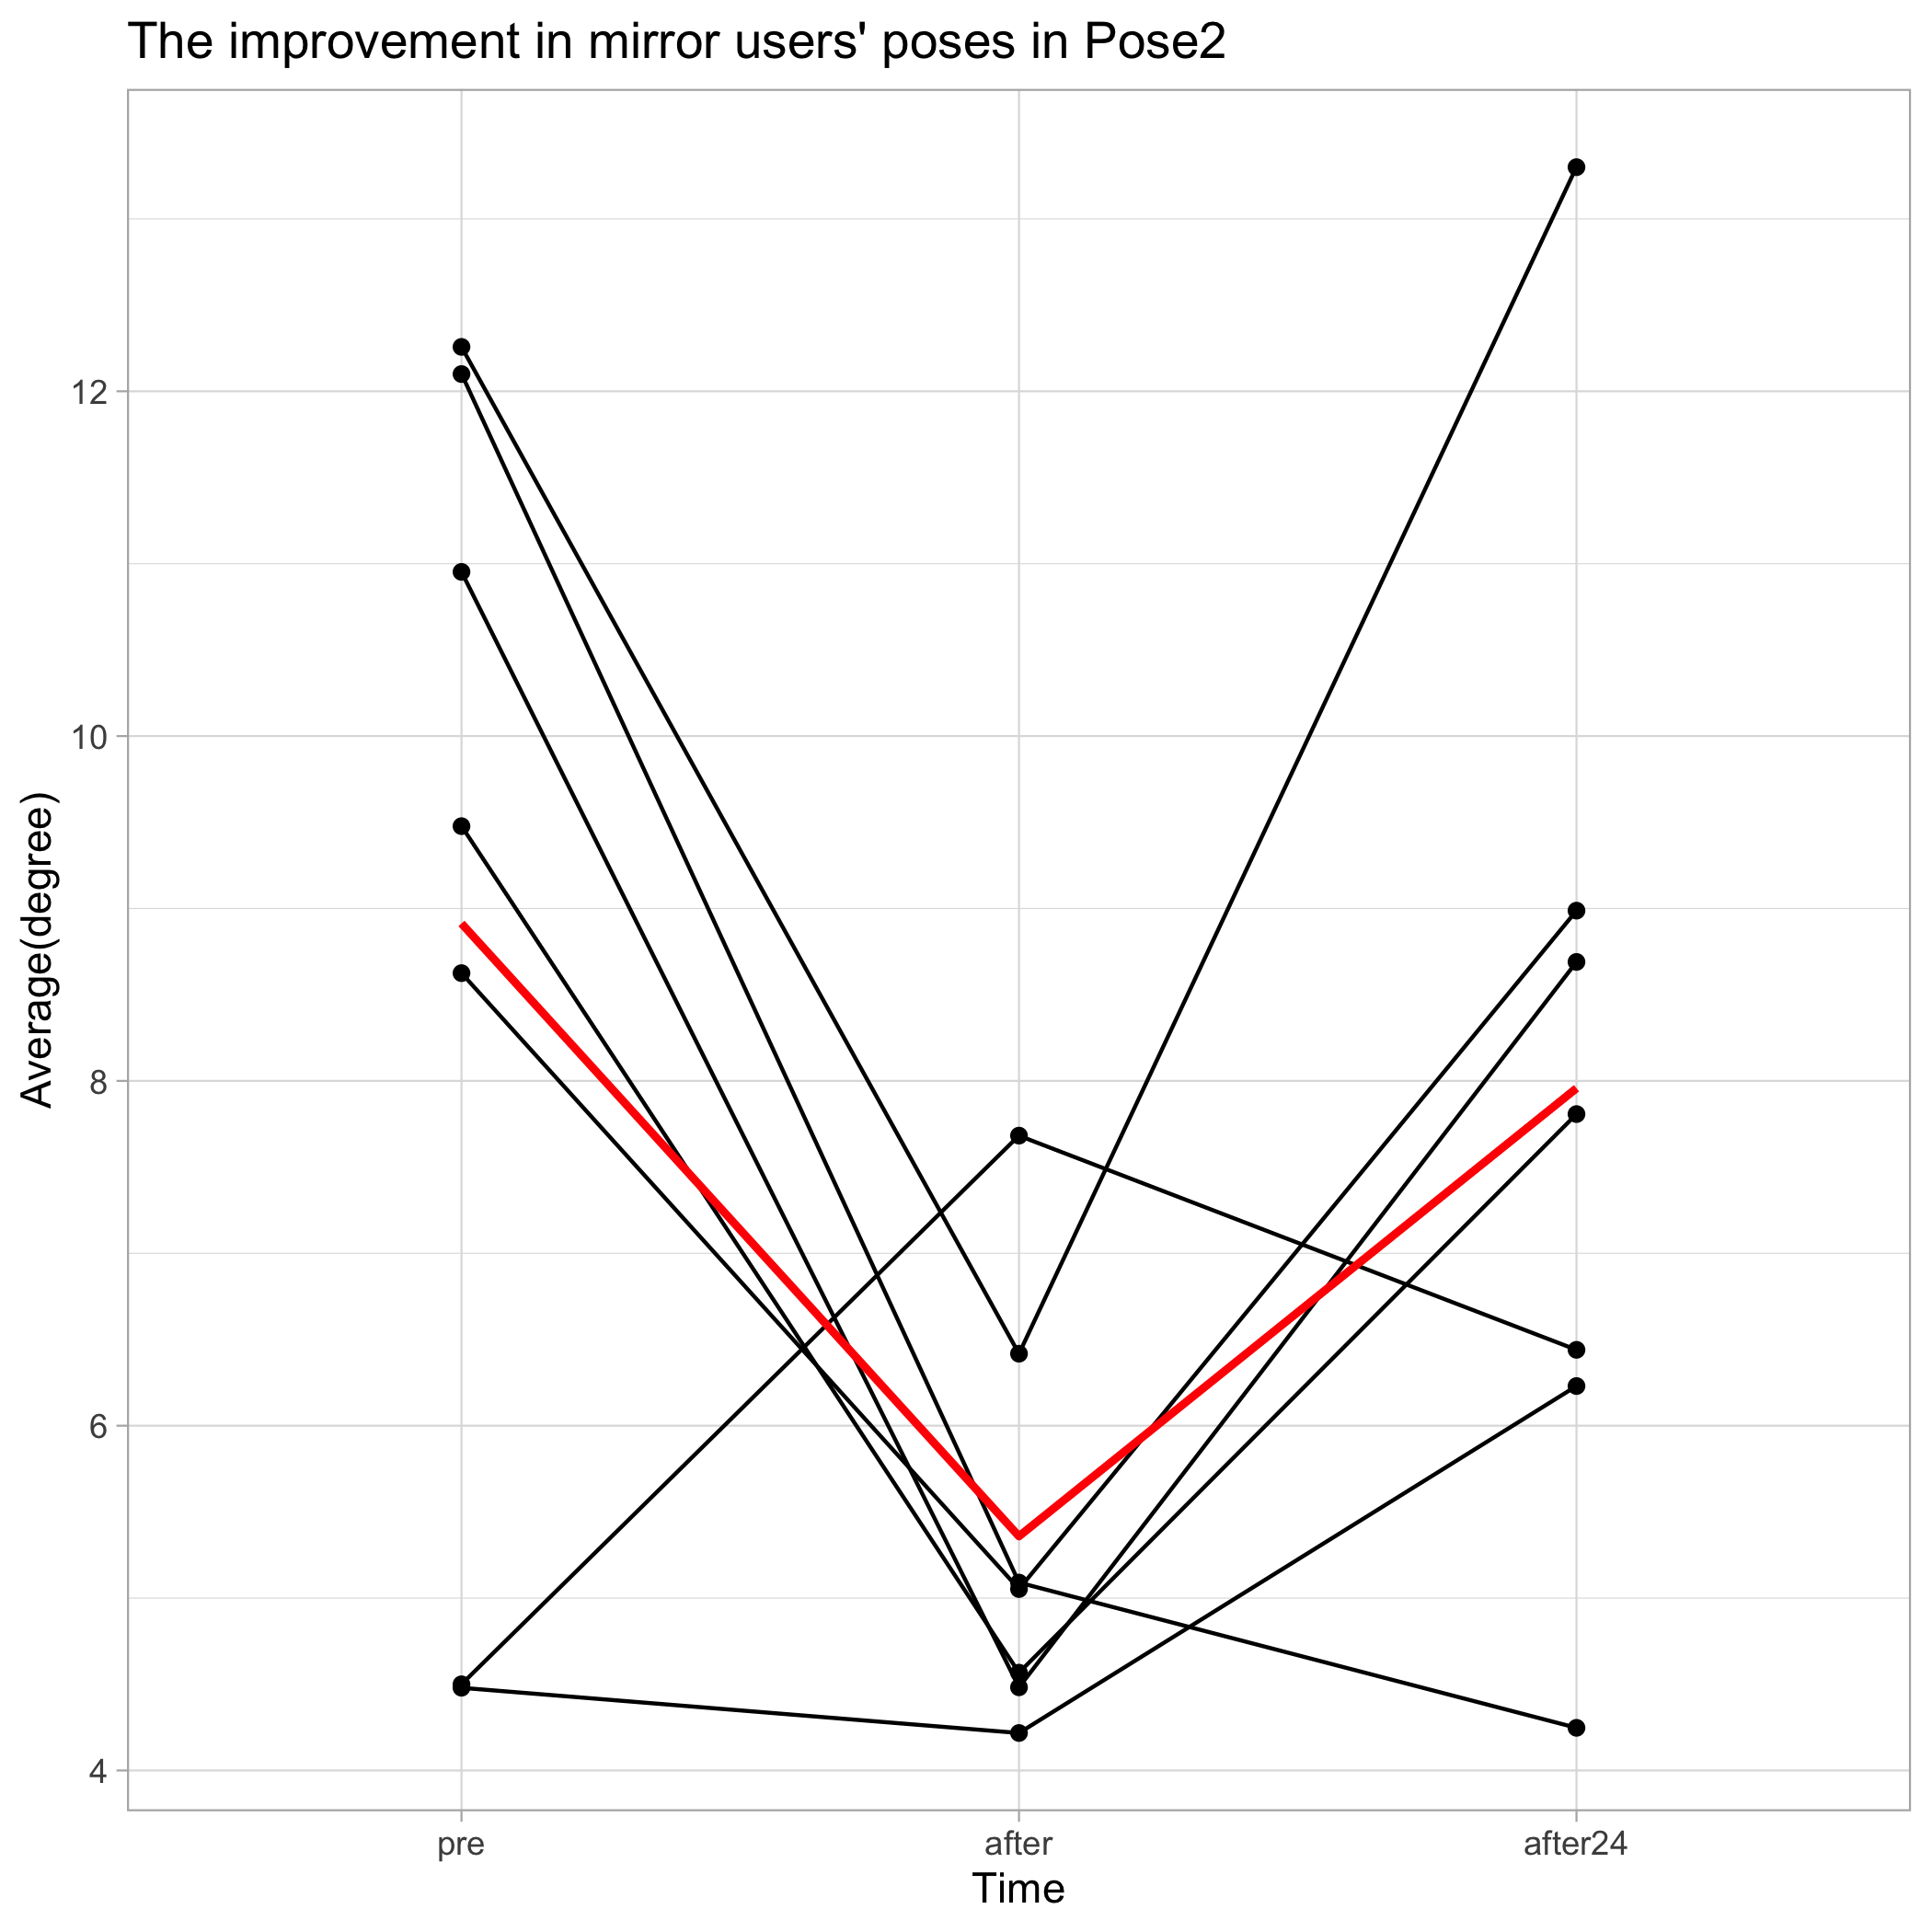
\includegraphics[width=9cm]{figures/pose2_system_false_graph.png}
        \caption{鏡利用群のpose2の結果}
        \label{fig:pose2_mirror}
        \end{center}
      \end{figure}

      \begin{table}[ht]
        \centering
        \caption{pose2における練習後、練習から24時間後と練習前の比較}
        \begin{tabular}{lcr}
        \hline
        \textbf{比較対象} & \textbf{p-value} & \textbf{MD} \\ \hline
        after-pre & 0.04688 & -3.554643 \\ \hline
        after24-pre & 0.8125 & -0.9557143 \\ \hline
        \end{tabular}
        \label{table:pose2_mirror_p_value}
        \end{table}

  \subsection{鏡利用群とシステム利用群の比較}
    ここでは同じポーズにおいてシステム利用群と鏡利用群の理想の角度との差の比較の結果を示す。

    \subsubsection{pose1における練習方法の違いによる比較}
      pose1に対してシステムを利用した群と鏡を利用した群の練習後の結果と理想の角度との差の平均\(\bar{\theta}_{\text{angle\_dif}}\)を図\ref{fig:pose1_after_practice}に、
      24時間後の比較を図\ref{fig:pose1_after24_practice}に示す。

      pose1においては、練習後の結果ではシステム利用群の方が鏡利用群よりもポーズが改善されていることがわかるが、p=0.7104と統計的に有意性を示すことができなかった。
      24時間後では表\ref{table:pose1_practice_p_value}にあるようにp=1と差を示すことができなかった。
      \begin{figure}[H]
        \begin{center}
        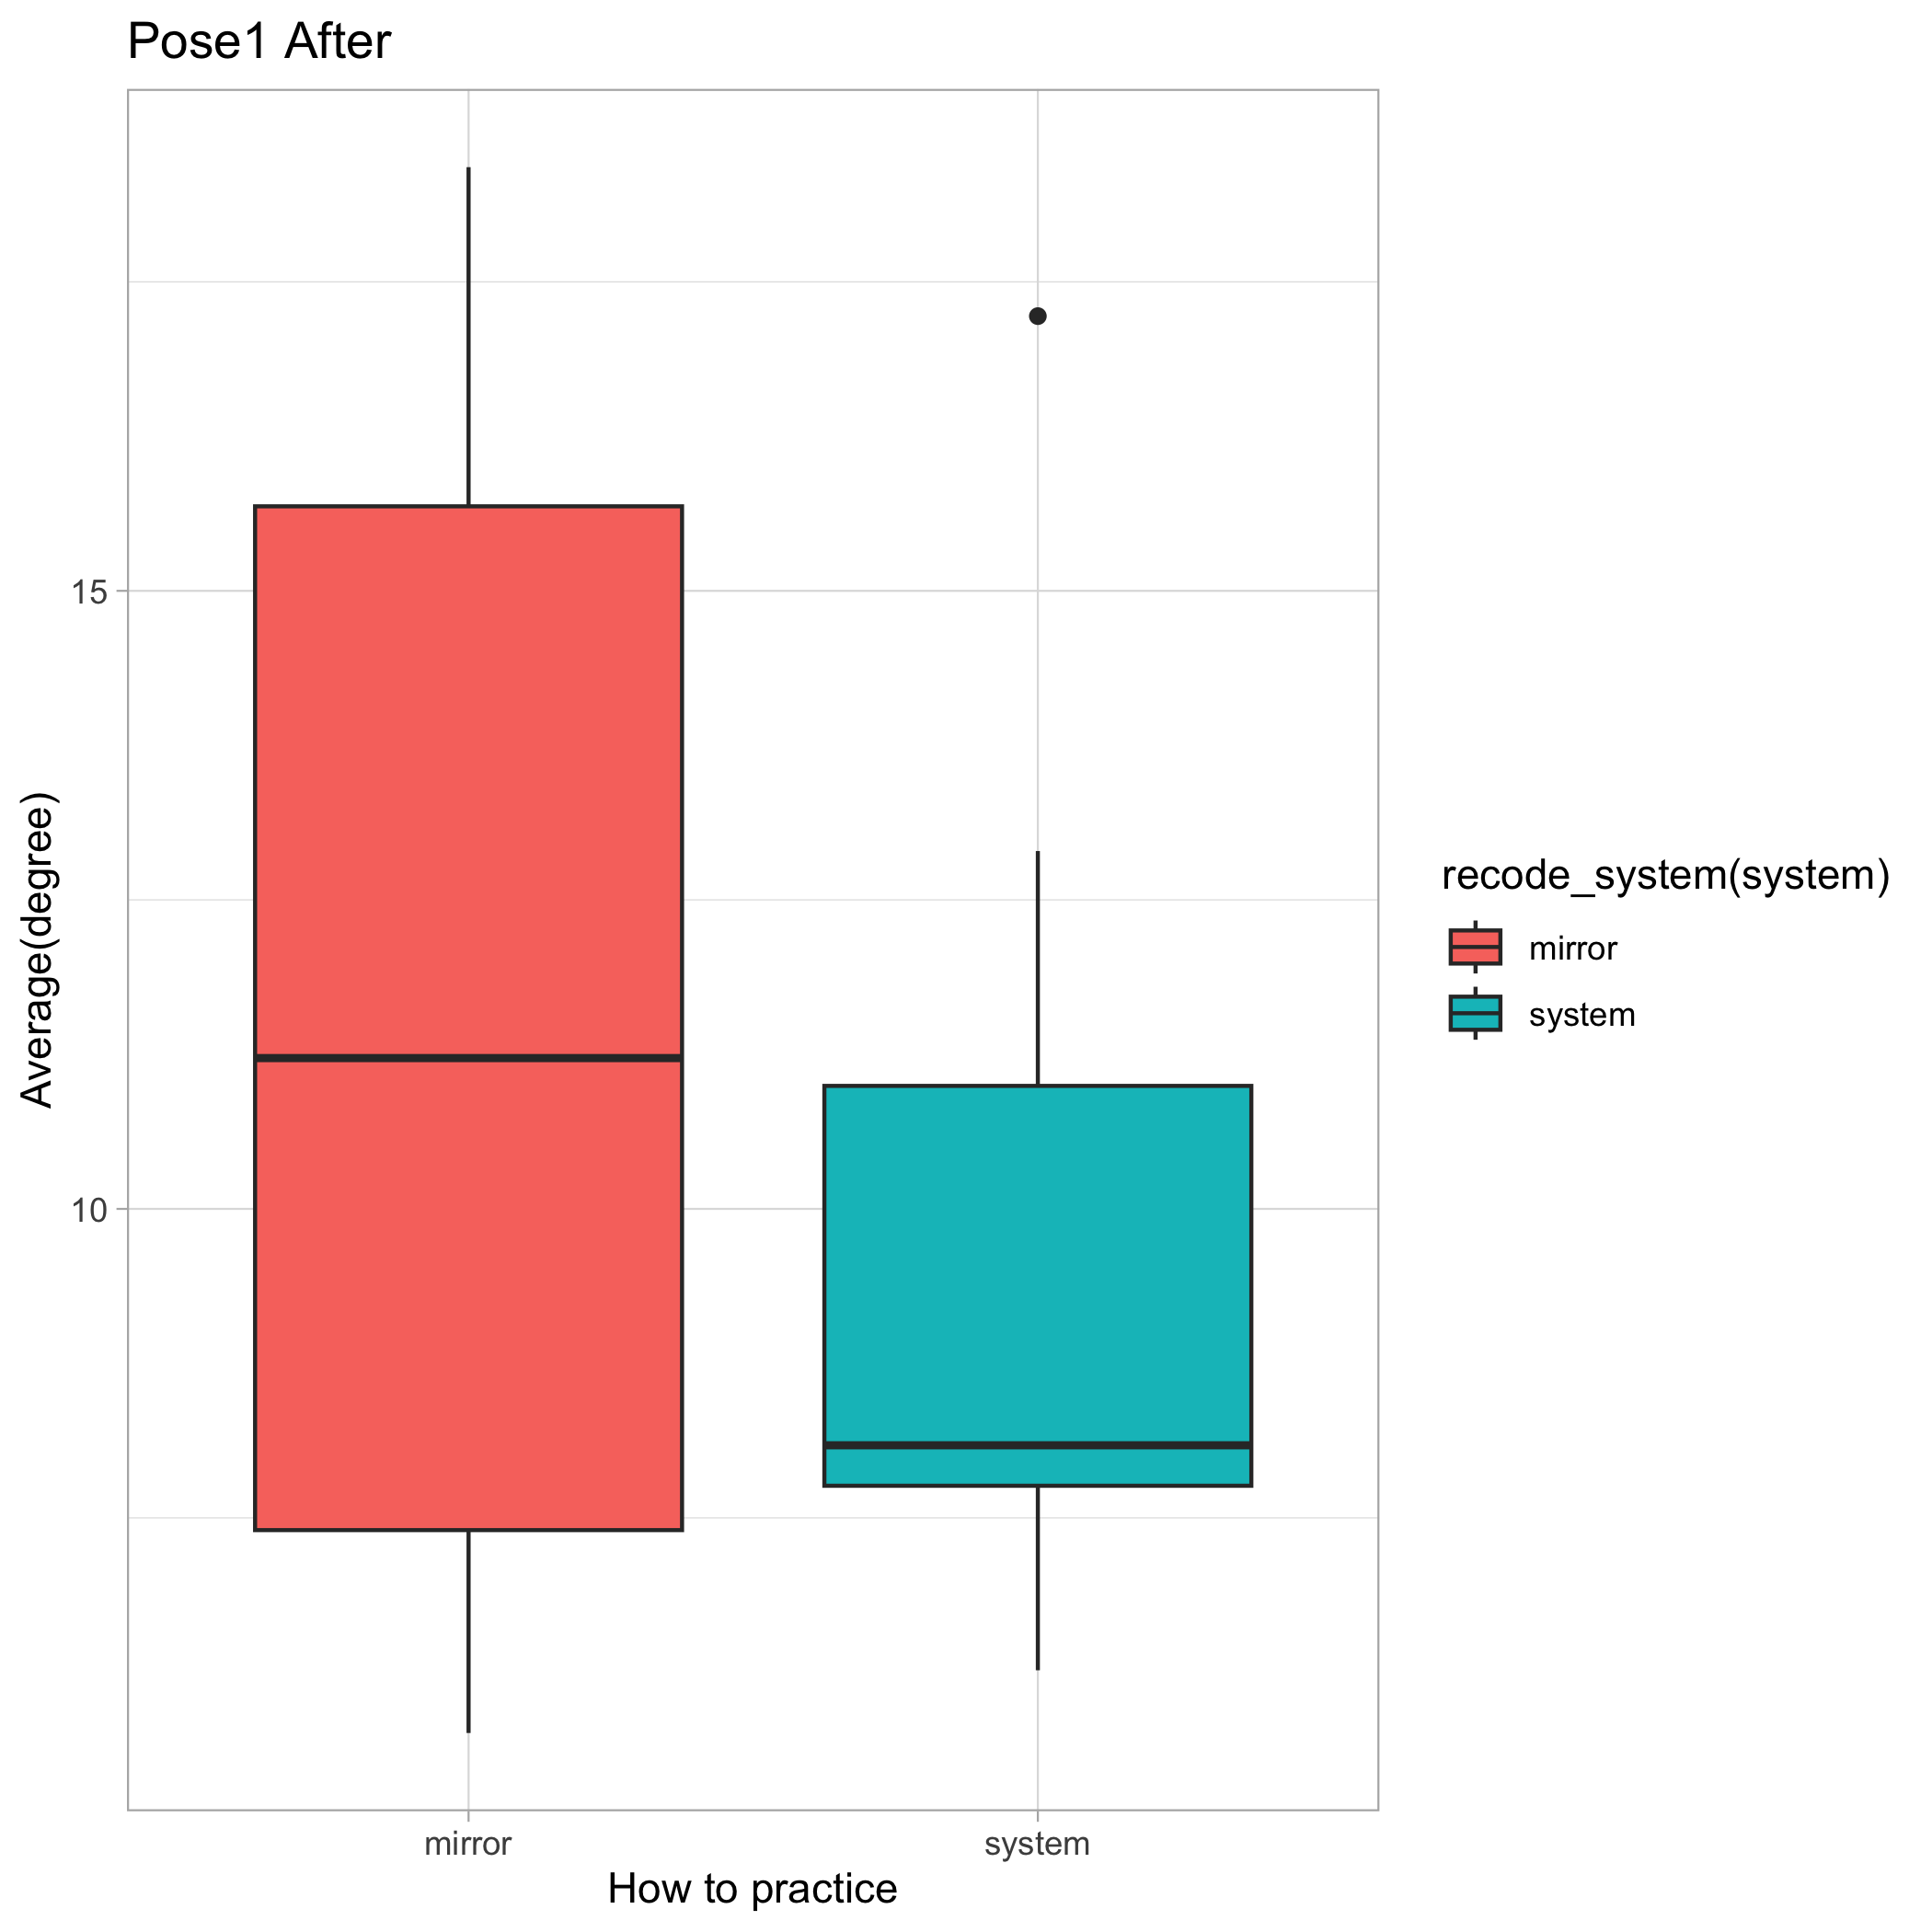
\includegraphics[width=9cm]{figures/pose1_after_boxplot.png}
        \caption{pose1における練習後の練習方法による比較}
        \label{fig:pose1_after_practice}
        \end{center}
      \end{figure}

      \begin{figure}[H]
        \begin{center}
        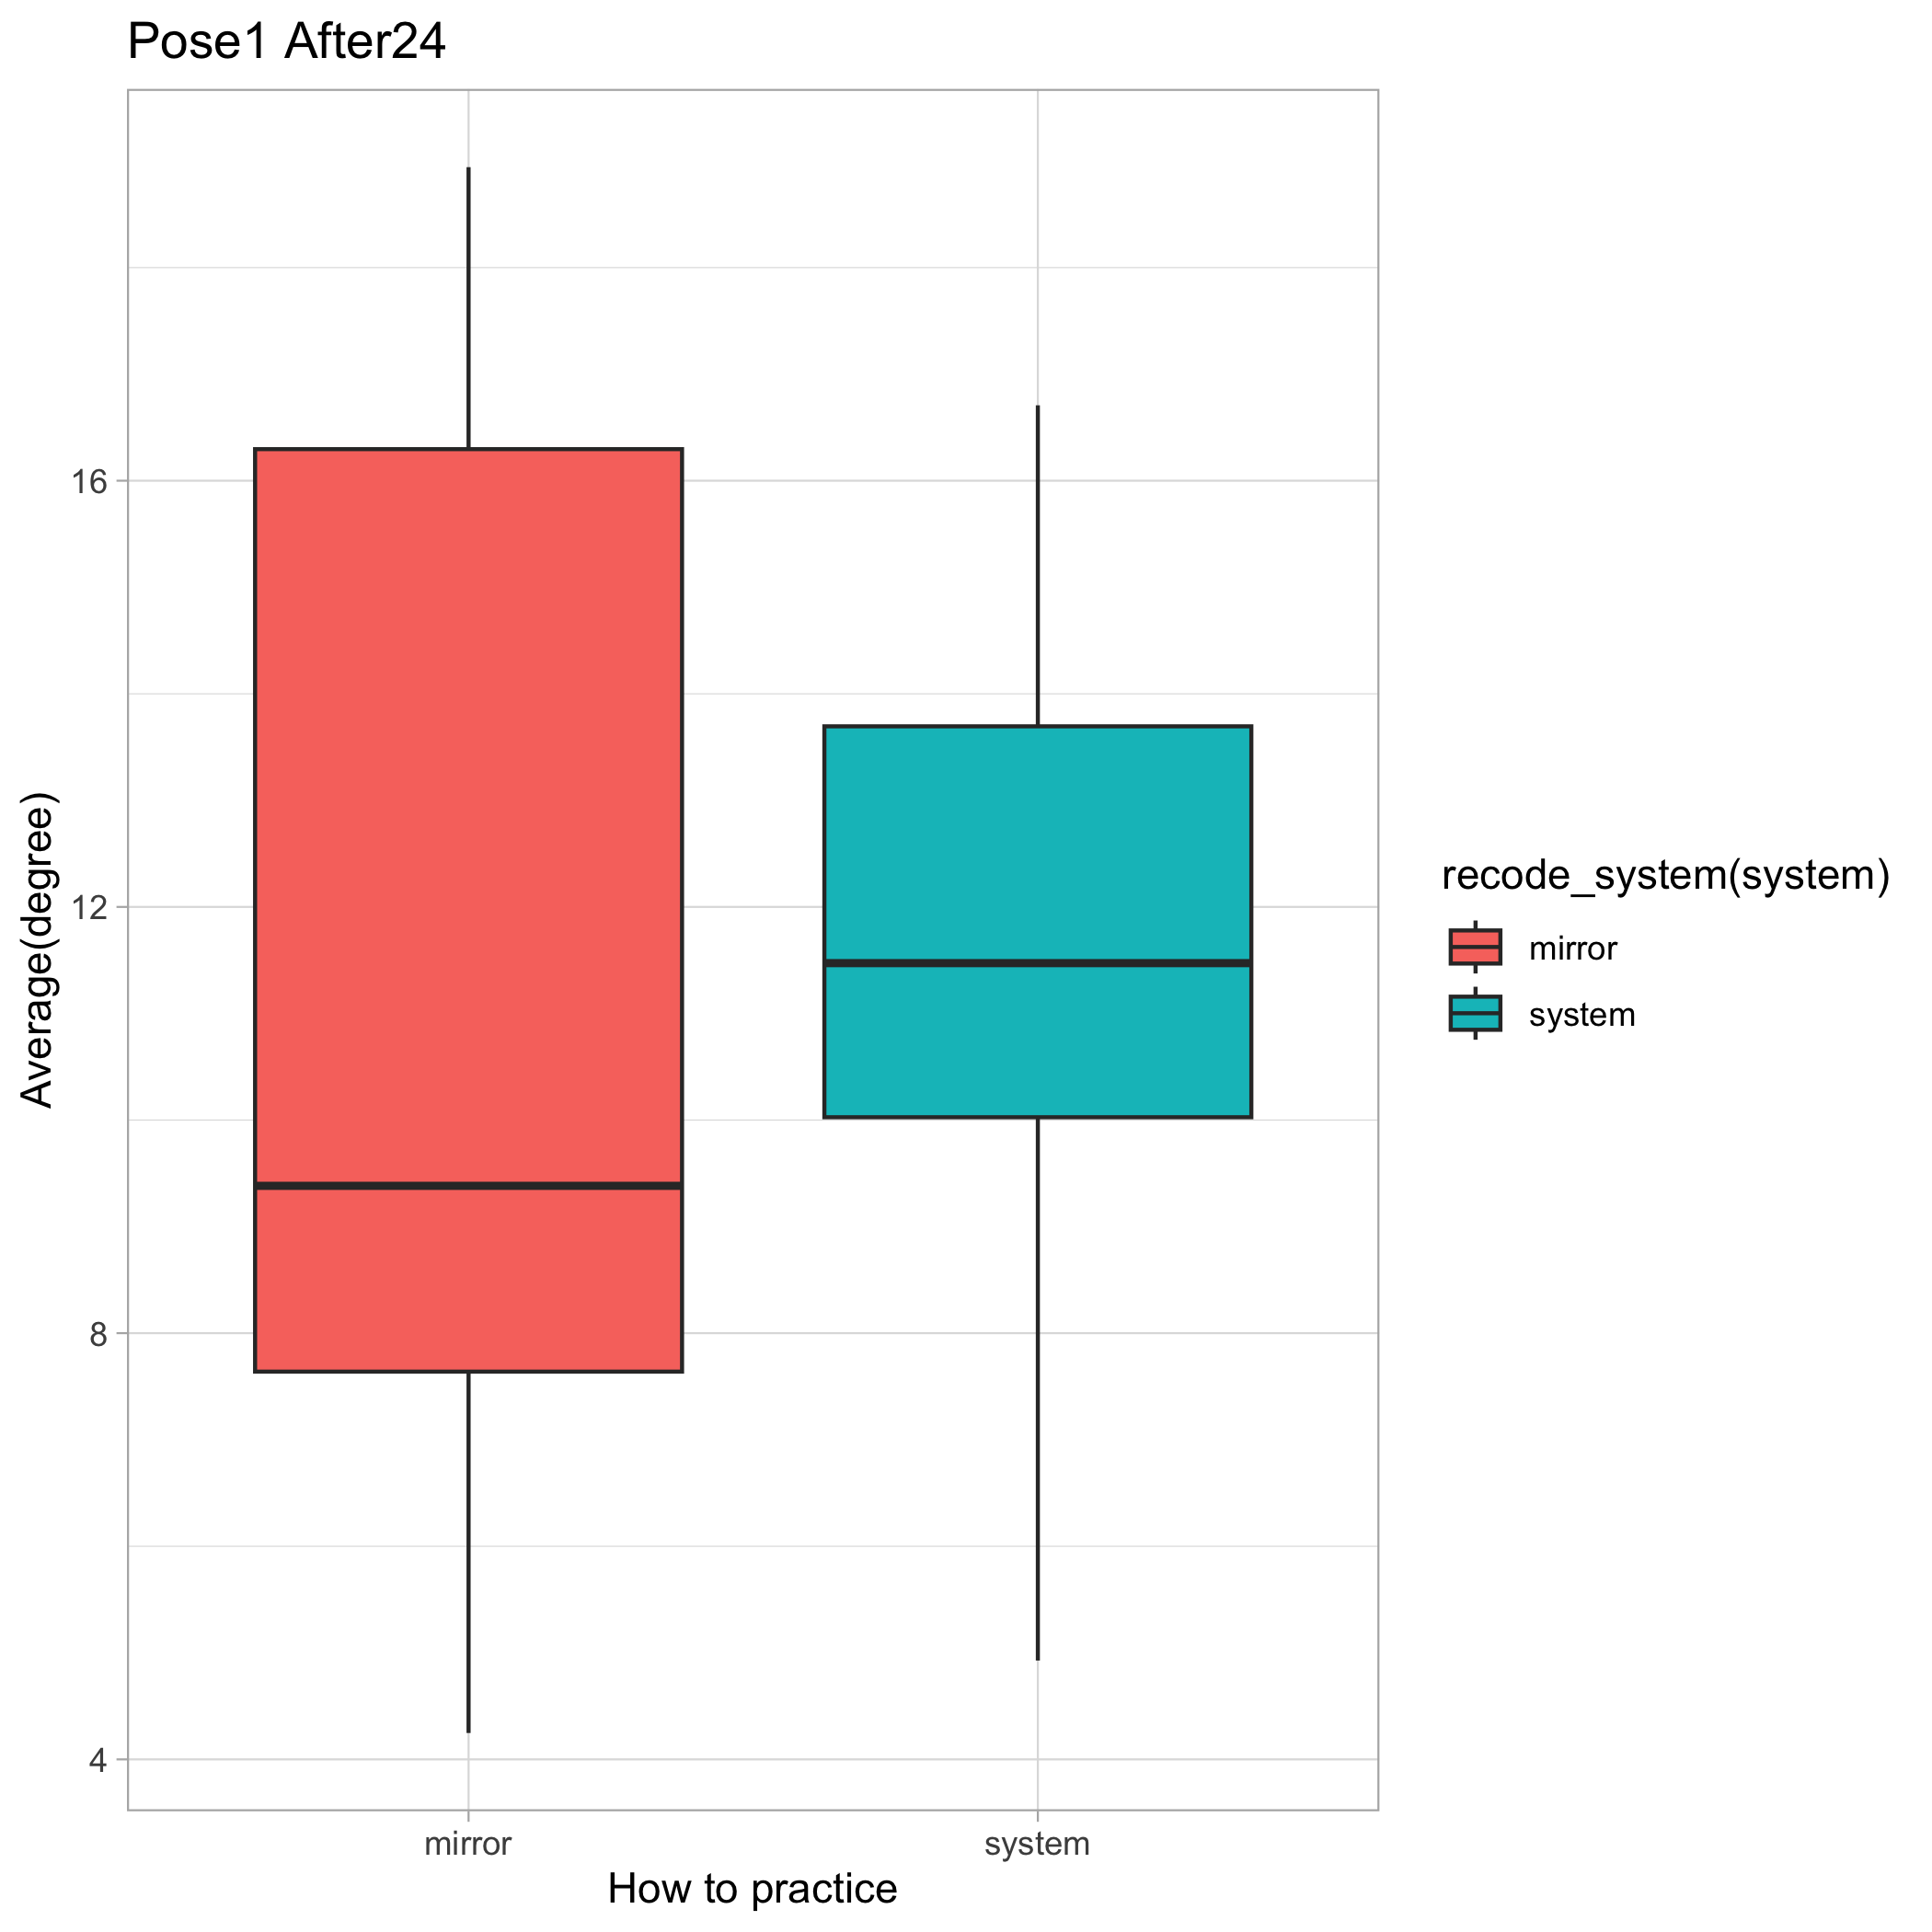
\includegraphics[width=9cm]{figures/pose1_after24_boxplot.png}
        \caption{pose1における24時間後の練習方法による比較}
        \label{fig:pose1_after24_practice}
        \end{center}
      \end{figure}

      \begin{table}[H]
        \centering
        \caption{pose1}
        \begin{tabular}{lcr}
        \hline
        \textbf{比較対象} & \textbf{p-value} & \textbf{平均差(システム-鏡)} \\ \hline
        after & 0.7104 & -1.784286\\ \hline
        after24 & 1 & 0.01535714\\ \hline
        \end{tabular}
        \label{table:pose1_practice_p_value}
        \end{table}
      
    \subsubsection{pose2における練習方法の違いによる比較}

      pose2に対してシステムを利用した群と鏡を利用した群の練習後の結果と理想の角度との差の平均\(\bar{\theta}_{\text{angle\_dif}}\)を図\ref{fig:pose2_after_practice}に、
      24時間後の比較を図\ref{fig:pose2_after24_practice}に示す。
      こちらでは表\ref{table:pose2_practice_p_value}に示すように統計的に有意とは言えないものの、pose1とは異なり練習後、24時間後ともに{\bf 鏡利用群の方が}システム利用群よりもポーズが改善されていることがわかる。
      \begin{figure}[H]
        \begin{center}
        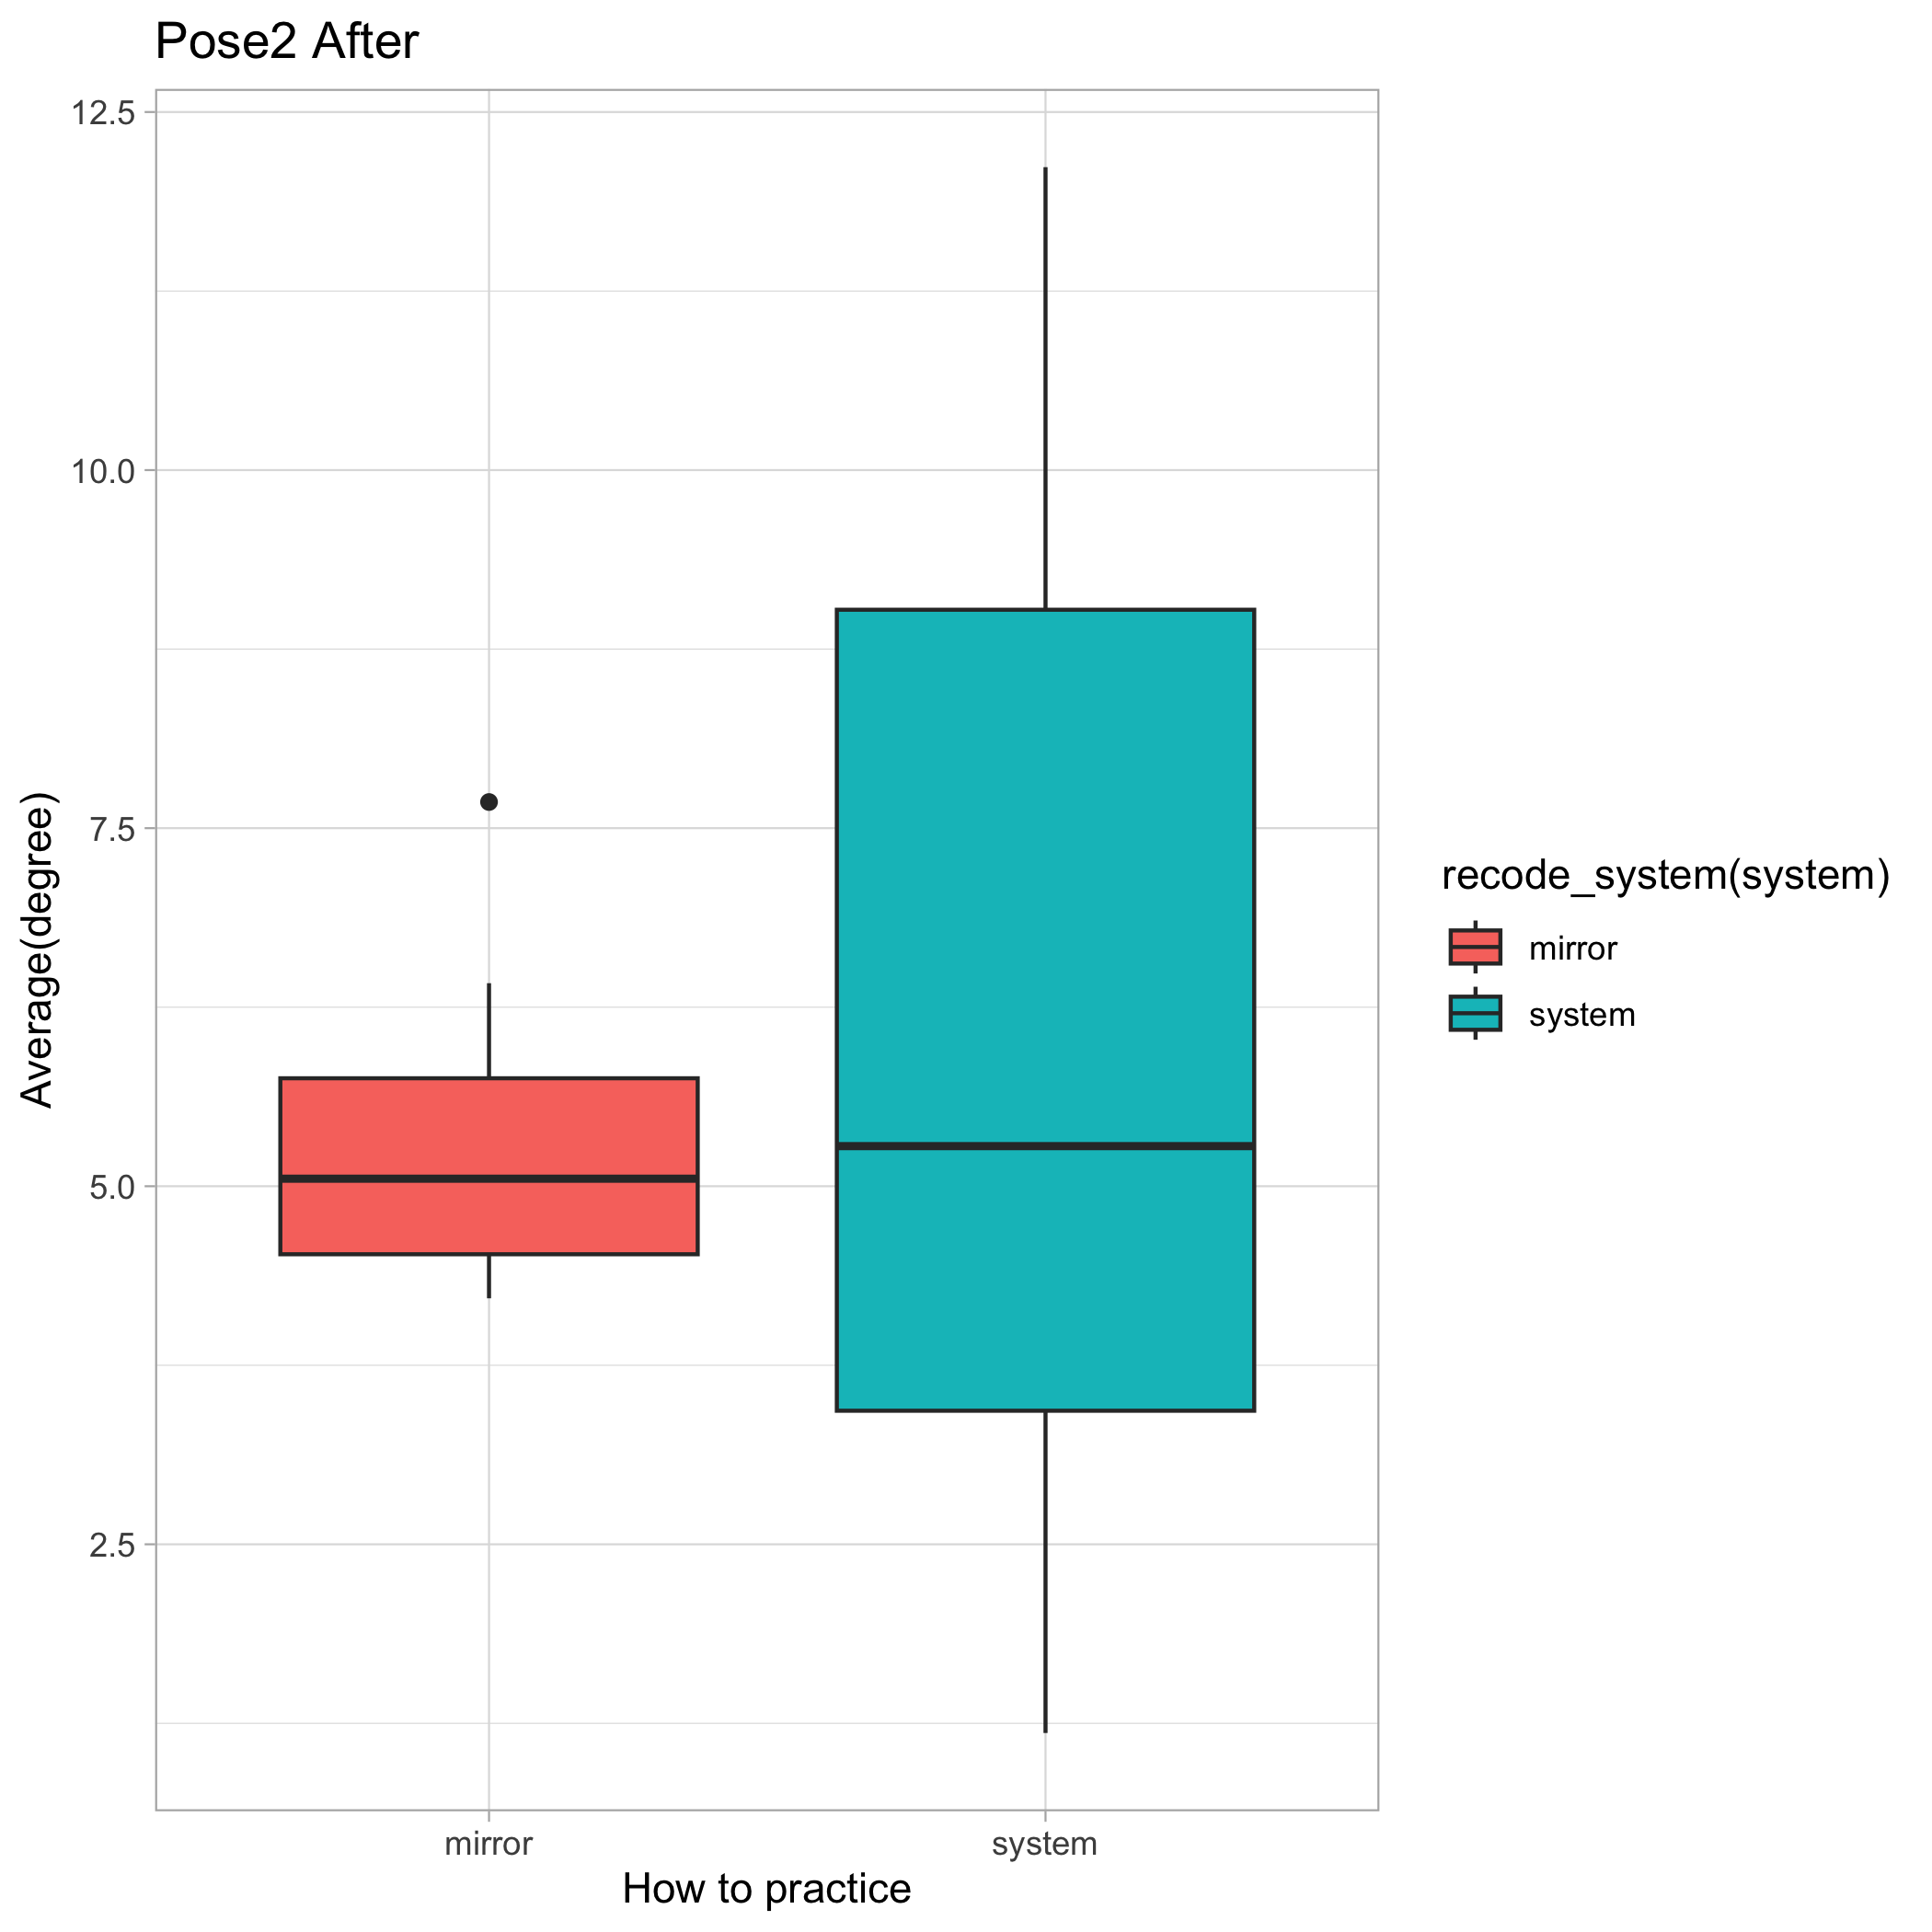
\includegraphics[width=9cm]{figures/pose2_after_boxplot.png}
        \caption{pose2における練習後の練習方法による比較}
        \label{fig:pose2_after_practice}
        \end{center}
      \end{figure}

      \begin{figure}[H]
        \begin{center}
        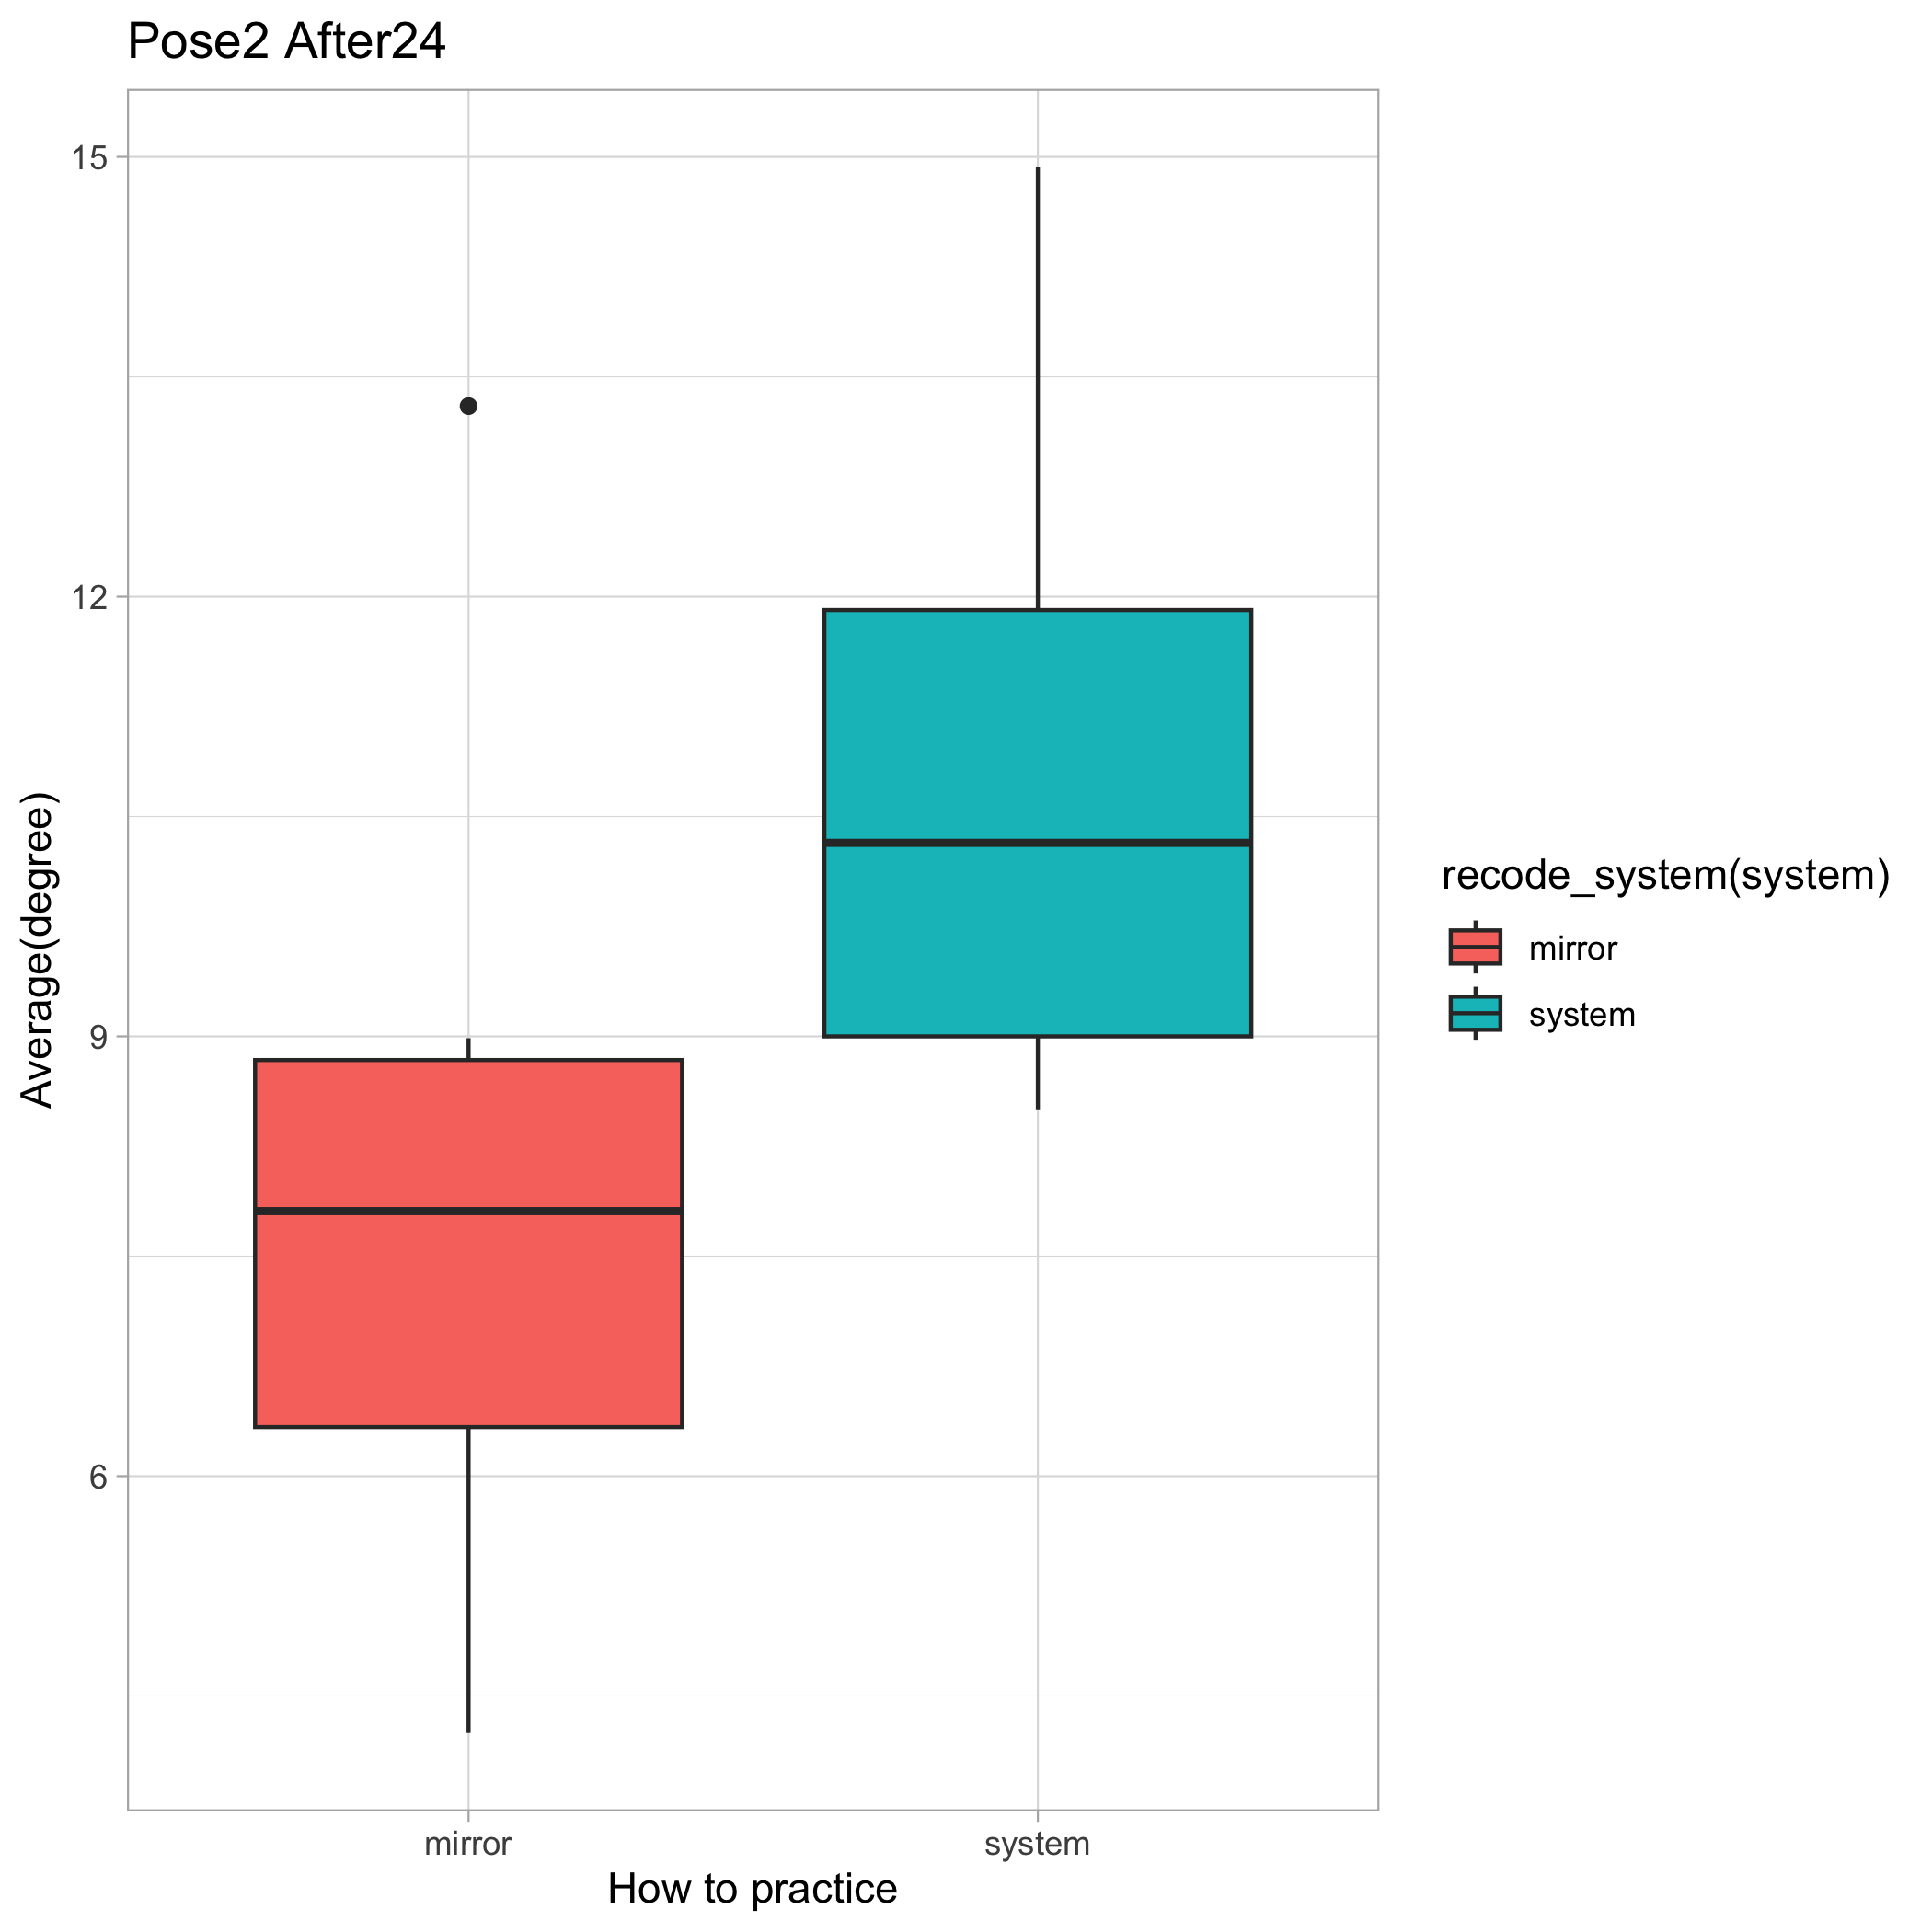
\includegraphics[width=9cm]{figures/pose2_after24_boxplot.png}
        \caption{pose2における24時間後の練習方法による比較}
        \label{fig:pose2_after24_practice}
        \end{center}
      \end{figure}

      \begin{table}[H]
        \centering
        \caption{pose2}
        \begin{tabular}{lcr}
        \hline
        \textbf{比較対象} & \textbf{p-value} & \textbf{平均差(システム-鏡)} \\ \hline
        after & 0.62 & 0.8546429 \\ \hline
        after24 & 0.07284 & 2.838214 \\ \hline
        \end{tabular}
        \label{table:pose2_practice_p_value}
        \end{table}



\input{src/7_conclusion}
%\input{src/appendix}
\chapter*{謝辞}
\addcontentsline{toc}{chapter}{謝辞}
\label{thanks}

本研究を進める過程で絶えずサポートをしてくださったRG(村井・中村・楠本・高汐・バンミーター・植原・三次・中澤・手塚・武田・大越合同研究会) の教員の方々、そしてメンバーの皆様には心からの感謝を申し上げます。特に、2020年秋学期に1年生の私を迎え入れてくださった慶應義塾大学大学SFC研究所の上席所員であり、早稲田大学商学学術院の教授である斉藤賢爾博士には、本研究に至るまでの丁寧なご指導に深く感謝します。

また、NECOのKGリーダーである江頭叙那氏、およびKGメンバーの皆様には、この貴重な研究グループに参加する機会を与えていただき、感謝の気持ちでいっぱいです。同様に、私がKGに参加するきっかけを作ってくれた卒業生、渡邉聡紀氏にも心からの謝意を表します。

この研究の実験にご協力いただいたRGのメンバーの方々、そして、母校である栃木県立宇都宮高校サッカー部のOBの皆様にも、貴重な時間を割いて協力していただいたことに深く感謝いたします。さらに、大学生活でボディビルの大会に挑戦するきっかけを作り、サポートとアドバイスをくださったバーベルクラブのメンバーとOBの皆様にも、心からの感謝を述べたいと思います。

そして、コロナ禍という厳しい時期に始まった大学生活を通じて、精神的に大きな支えとなってくれた渡邉美穂氏に、特別な感謝の意を表します。

最後になりましたが、私の成長を見守り、学びの場を提供してくれた両親をはじめとする家族に、最大の感謝の気持ちを捧げます。



%%% Local Variables:
%%% mode: japanese-latex
%%% TeX-master: "../yummy_bthesis"
%%% End:


\renewcommand{\thechapter}{\Alph{chapter}}
\setcounter{chapter}{0}
\vspace{-5mm}


\input{bib/biblio}\thispagestyle{plain}%bibtex


\end{document}

%%% Local Variables:
%%% mode: japanese-latex
%%% TeX-master: t
%%% End:
